\documentclass[uplatex, a4paper, 12pt, openany, oneside]{jsbook}

\usepackage[dvipdfmx]{graphicx}
\usepackage[dvipdfmx]{color}
\usepackage[dvipdfmx, bookmarks=true, setpagesize=false, hidelinks]{hyperref}
\usepackage{pxjahyper}

\usepackage{thesis}
\usepackage{here}
\usepackage{url}


\thesis{修 士 論 文}
\title{
  \centering
    \scalebox{1.0}{オープンプラットフォームオフィスロボットの開発}\\
    \vspace{-0.5zh}
    \scalebox{0.9}{-QDDモータを使用した}\\
    \vspace{-0.7zh}
    \scalebox{0.9}{ロボットアームのメカニズムの設計と製作-}\\
    \vspace{0.4zh}
    \scalebox{0.8}{Development of Open Platform Office Robot}\\
    \vspace{-1.0zh}
    \scalebox{0.7}{-Design and Construction of a Robot Arm Mechanism}\\
    \vspace{-1.0zh}
    \scalebox{0.7}{using QDD Motor-}
    \vspace{-3zh}
}
\setlength{\textwidth}{\fullwidth}
\setlength{\evensidemargin}{\oddsidemargin}

\date{\today}
\vspace{-10.0zh}
\teacher{林原 靖男 教授}
\vspace{-10.0zh}
\organization{千葉工業大学 先進工学研究科 未来ロボティクス専攻}
\author{23S1008 川鍋清志郎}
\vspace{-10zh}

\renewcommand{\baselinestretch}{1.2}
\begin{document}

%% Front Matter
\frontmatter{}
%
\chapter{設計}
\label{chap:third}
%
本章ではロボットアームのメカニズムの設計について述べる.
まず,選定したQDDモータについて説明し,ロボットアームの設計について述べる.

%!TEX root = ../thesis.tex
\section{オープンプラットフォームを意識した設計}
\newpage
%!TEX root = ../thesis.tex
\section{QDDモータの選定}
飯塚ら\cite{飯塚浩太2021}の研究では,減速比10:1のQDDモータが使用されている.また,Zhaoら\cite{10106520}の研究においては,減速比9:1のQDDモータが採用されていた.これらの先行研究は,ロボットアームと人の衝突時の衝撃力軽減を実現するためには,この程度の減速比を持つモータを採用することが有効であることを示唆している.

さらに,本研究ではオープンプラットフォームの観点を重視し,他のロボットアームに使用されているモータと同程度,またはそれ以下の価格であることを選定基準とした.調査対象としたオフィスロボットのうち,ロボットアームに使用しているアクチュエータの価格は,約3万円から約8万円であったため,価格上限を8万円に設定した.

以上を踏まえ,本研究では,持つSteadywinのGIM8108-8とGIM3505-8を採用した.減速比は8:1であり,先行研究で使用されていたモータと同程度の減速比を持つ.また,価格は約19,000円と約18,000円であり,価格上限である8万円を下回っている.
\subsection{選定したモータの性能}
表\ref{tab:QDDComparison}に,選定したQDDモータとReachy\cite{Reachy:online}のアームに使用されているモータ(Dynamixel MX-106T)の比較を示す.選定したSteadywinのGIM8108-8とGIM3505-8は,減速比が8:1で,先行研究で使用していた減速比と近しい物になっている.適切に制御することで衝突時の衝撃を軽減することが可能である.また,許容ラジアル荷重とアキシアル荷重も高いため,追加の補強部品を必要とせずにロボットアームの構造を簡略化することが可能である.
\begin{table}[]
  \centering
  \caption{QDD motor performance comparison}
  \label{tab:QDDComparison}
  \begin{tabular}{lccc}
  \hline
               & \begin{tabular}[c]{@{}c@{}}SteadyWin\\ GIM8108-8\end{tabular} & \begin{tabular}[c]{@{}c@{}}SteadyWin\\ GIM3505-8\end{tabular} & \begin{tabular}[c]{@{}c@{}}Dynamixel\\ MX-106T\end{tabular} \\ \hline
  減速比          & 8 : 1                                                         & 8 : 1                                                         & 225 : 1                                                     \\
  定格トルク(Nm)    & 7.5                                                           & 0.65                                                          & -                                                           \\
  最大トルク(Nm)    & 22                                                            & 1.27                                                          & 10                                                          \\
  重量(g)        & 396                                                           & 97                                                            & 153                                                         \\
  無負荷回転数(rpm)  & 320                                                           & 384                                                           & 55                                                          \\
  許容ラジアル荷重(N)  & 900                                                           & 300                                                           & 40                                                          \\
  許容アキシアル荷重(N) & 225                                                           & 75                                                            & 20                                                          \\
  価格(円)        & 約19,000                                                       & 約18,000                                                       & 約80,000                                                     \\ \hline
  \end{tabular}
\end{table}

\subsection{QDDモータの欠点}
QDDモータは高トルク・高スピードでの動作が可能であるという利点を持つ一方で、この特性は制御が不十分な場合にリスクとなる.特に、通電時に動作が暴走した場合、一般的なモータと比較して周囲の人や機器への被害が大きい.そのため、QDDモータを安全に運用するためには、適切な制御と安全対策が必要である.
\newpage
%!TEX root = ../thesis.tex
\section{基本的な性能}
設計したロボットアームの基本的な性能を述べる.
\subsection{アームサイズ}
図\ref{fig:link_length}にロボットアームのアームリーチとリンク長を示す.人間の腕の長さの比\cite{humanarm:online}を参考に,肩から肘までは290㎜,肘から手首までは220㎜とした.アームリーチは660㎜であり,要求仕様の700㎜程度を満たしている.図\ref{fig:arm_size}にアームサイズを示す.比較のため,机とボトルを模したものを配置している.

\begin{figure}[htbp]
  \centering
  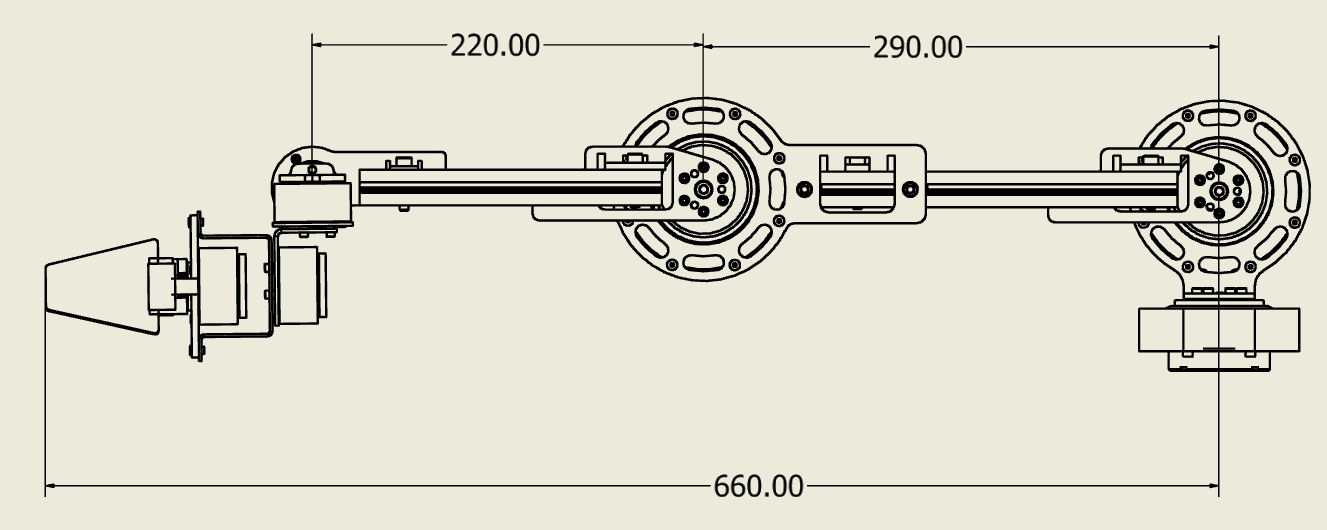
\includegraphics[width=10cm]{images/link_length.png}
  \caption{Arm reach and link length}
  \label{fig:link_length}
\end{figure}

\begin{figure}[htbp]
  \centering
  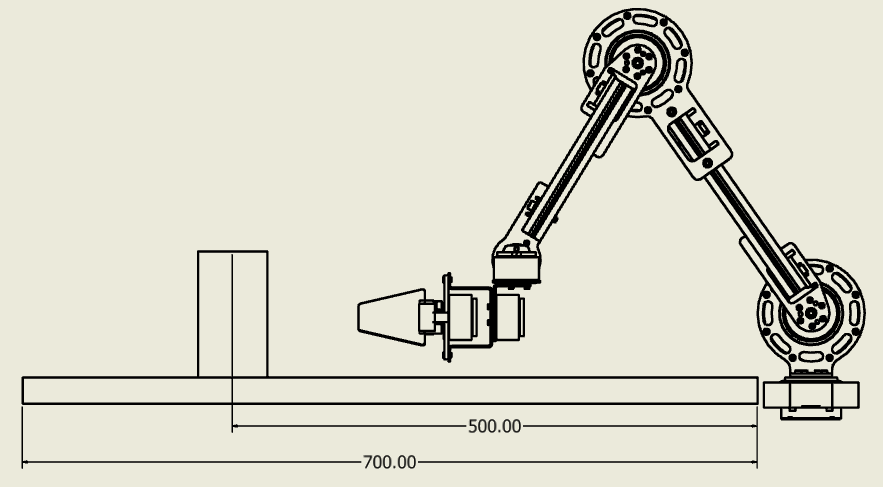
\includegraphics[width=10cm]{images/hikaku.png}
  \caption{Arm size}
  \label{fig:arm_size}
\end{figure}

\clearpage

\subsection{可動範囲}
図\ref{fig:arm_short},図\ref{fig:arm_long}にアームの最小可動範囲と最大可動範囲を示す.最小可動範囲は,アームの部品が干渉することなく動作できる最小の範囲を示しており,最大可動範囲はアームを最大まで伸ばしたときの範囲を示している.

\begin{figure}[htbp]
  \centering
  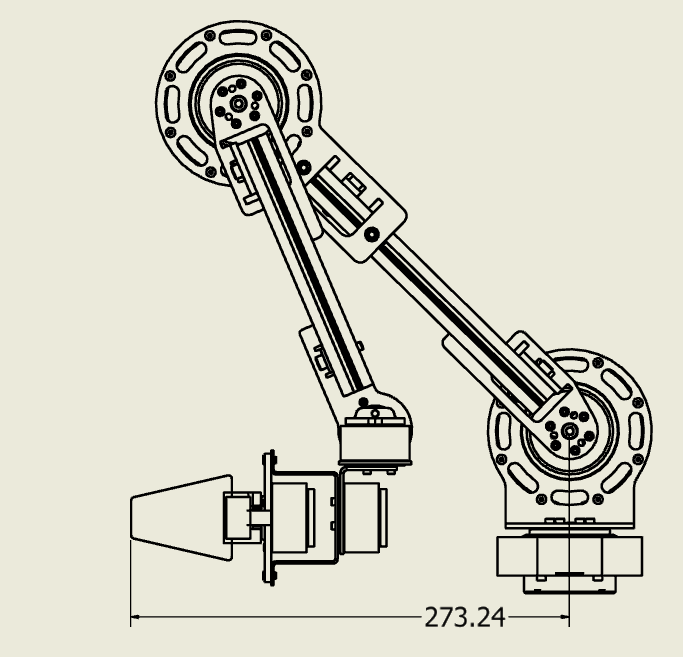
\includegraphics[width=10cm]{images/design/arm_short.png}
  \caption{Minimum range of motion}
  \label{fig:arm_short}
\end{figure}

\begin{figure}[htbp]
  \centering
  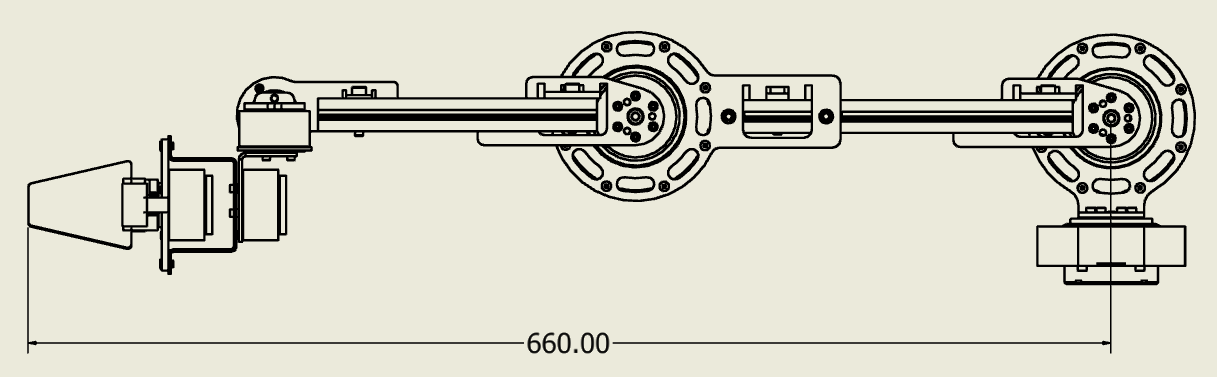
\includegraphics[width=10cm]{images/design/arm_long.png}
  \caption{Minimum range of motion}
  \label{fig:arm_long}
\end{figure}

\subsection{アームの手先の移動}
アームの手先の移動の様子を図\ref{fig:move1},図\ref{fig:move2},図\ref{fig:move3},図\ref{fig:move4}に示す.

\begin{figure}[h]
  \centering
  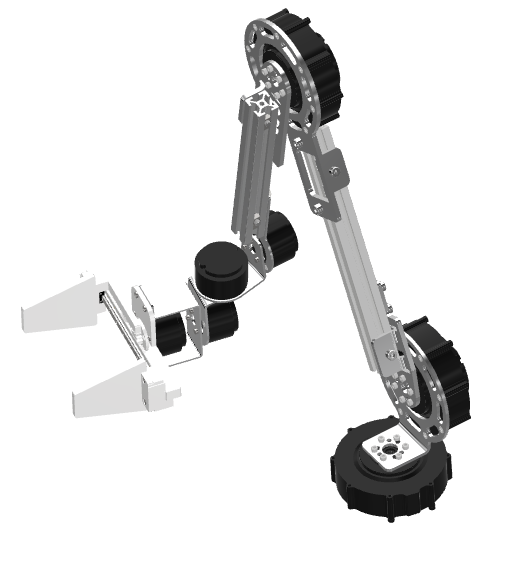
\includegraphics[width=10cm]{images/design/migitika.png}
  \caption{Stretched out to the right}
  \label{fig:move1}
\end{figure}

\begin{figure}[h]
  \centering
  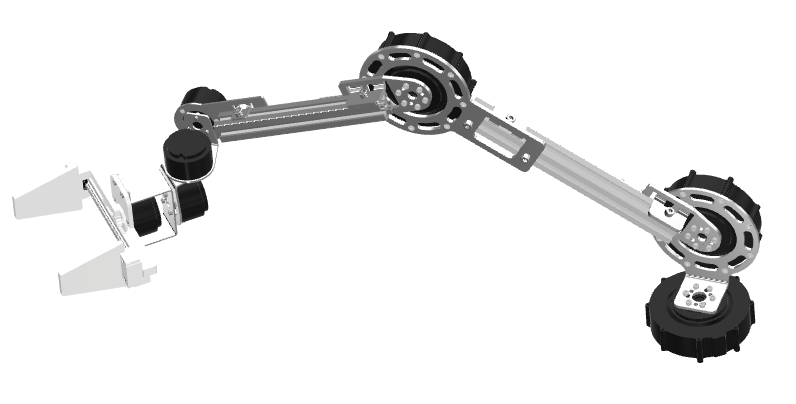
\includegraphics[width=10cm]{images/design/migioku.png}
  \caption{Stretched out to the right}
  \label{fig:move2}
\end{figure}

\begin{figure}[h]
  \centering
  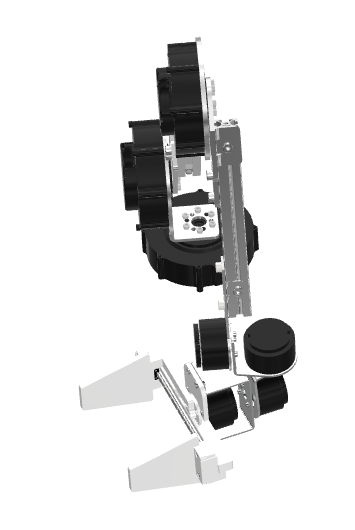
\includegraphics[width=8cm]{images/design/hidaritika.png}
  \caption{Stretched out to the left}
  \label{fig:move3}
\end{figure}

\begin{figure}[h]
  \centering
  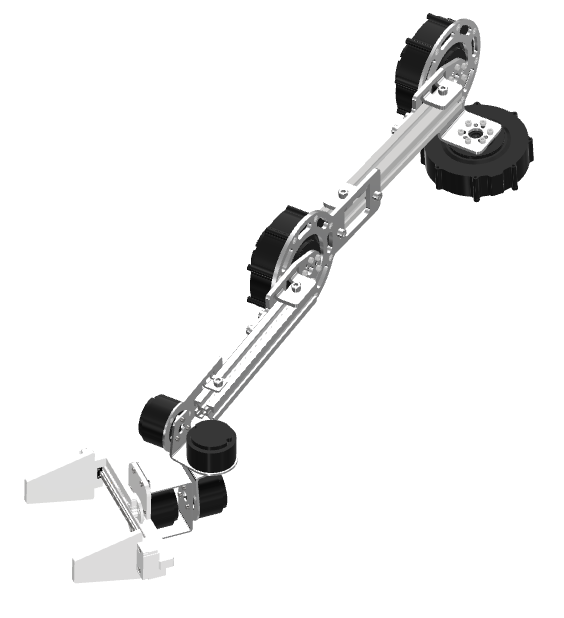
\includegraphics[width=10cm]{images/design/hidarioku.png}
  \caption{Stretched out to the left}
  \label{fig:move4}
\end{figure}
\clearpage

\subsection{可搬重量}
肩ピッチ軸のQDDモータ(SteadyWin GIM8108-8)の定格トルクは7.5Nm,最大トルクは22Nmである.アームを伸ばしたときに自重を支えるために必要なトルクを求め,常時把持することのできる物体の重量と,瞬間的に把持することのできる物体の重量を求める.
\subsubsection{自重を支える為に必要なトルク}
図\ref{fig:CoG}にアームの重心を示す.アームの重心は肩ピッチ軸から0.334mの位置にあり,アームの重さは1.31kgである.重力加速度を9.8m/s$^2$とすると,肩ピッチ軸にかかるトルク$T$は次のように求められる.
\begin{equation}
  T = 1.31 \times 9.8 \times 0.334 = 4.2 Nm
\end{equation}
\begin{figure}[h]
  \centering
  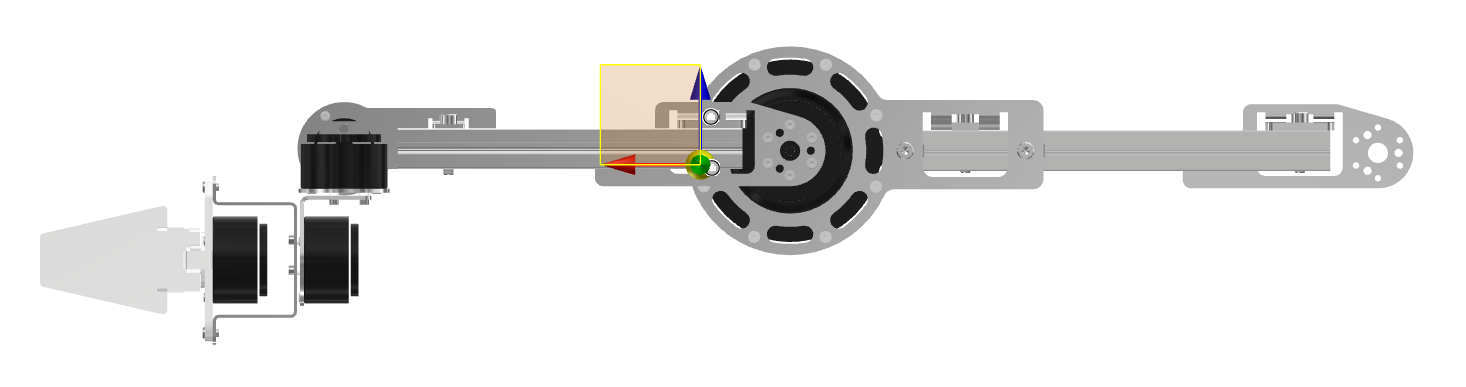
\includegraphics[width=10cm]{images/design/CoG.png}
  \caption{Center of gravity}
  \label{fig:CoG}
\end{figure}

\subsubsection{常時把持することのできる物体の重量}
アームの定格トルクから,自重を支える為に必要なトルクを引くと3.3Nmであり,肩ピッチ軸から手先までの距離は0.66mである.したがって,常時把持することのできる物体の重量$m$は次のように求められる.
\begin{equation}
  m = 3.3 / (9.8 \times 0.66) = 0.51kg
\end{equation}

\subsubsection{瞬間的に把持することのできる物体の重量}
同様に,最大トルクから自重を支える為に必要なトルクを引くと17.8Nmである.したがって,瞬間的に把持することのできる物体の重量$M$は次のように求められる.
\begin{equation}
  m = 17.8 / (9.8 \times 0.66) = 2.75kg
\end{equation}


\clearpage
\newpage
%!TEX root = ../thesis.tex
\section{強度確認}
設計したロボットアームの強度確認のため,Autodesk Inventorの機能である構造解析を行った.解析における安全率が1以上であれば,強度が十分であると判断した.図\ref{fig:shoulder}に肩部の構成を示す.肩部は,ヨー軸モータとピッチ軸モータを繋ぐ図\ref{fig:shoulder}の部品1,およびリンクの一部である,部品2から構成されている.部品1および部品2には,いずれもアルミニウム合金(A5052)を使用している.

本節では,構造解析による部品の強度確認について述べる.

\begin{figure}[h]
  \centering
  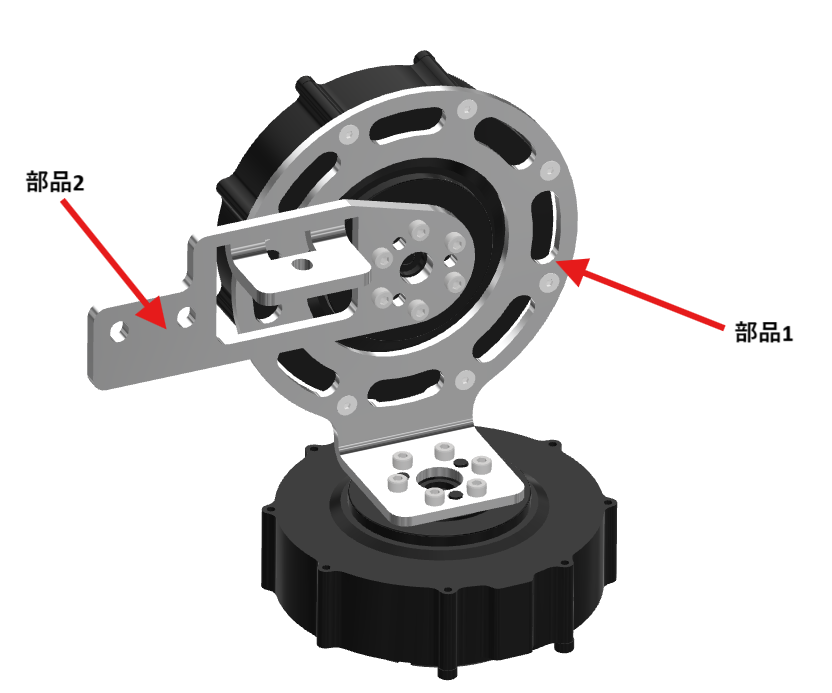
\includegraphics[width=10cm]{images/design/shoulder.png}
  \caption{Configuration of the shoulder components}
  \label{fig:shoulder}
\end{figure}

\subsection{部品1の構造解析}
図\ref{fig:shoulder}の部品1は,ヨー軸モータが最大出力22Nmを発生した際に最大負荷を受ける部品である.図\ref{fig:T3_40}に構造解析結果を示し,設計仕様を表\ref{tab:part1_spec}にまとめた.解析の結果,安全率は0.39であり,強度が不足していることが確認された.特に,図\ref{fig:T3_40}の結果から,曲げ加工部分において強度が不足していることが明らかとなった.この課題を解決するため,「板厚を変更した部品」と「形状を変更した部品」の2つの設計案を検討し,それぞれ再解析を実施した.

\begin{figure}[h]
  \centering
  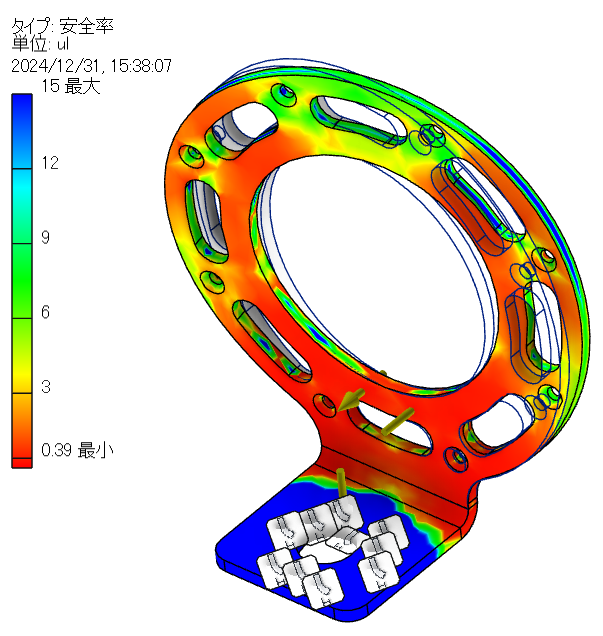
\includegraphics[width=6cm]{images/design/T3_40.png}
  \caption{Structural analysis results of Part 1}
  \label{fig:T3_40}
\end{figure}

\begin{table}[h]
  \centering
  \caption{Specifications of Part 1}
  \begin{tabular}{lc}
    \hline
    厚み & 3㎜ \\ 
    質量 & 43.6g \\ 
    安全率 & 0.39 \\ \hline
  \end{tabular}
  \label{tab:part1_spec}
\end{table}
\clearpage

\subsection{設計の変更}
部品の形状はそのままに,板厚を3mmから5mmに変更した場合の構造解析結果を図\ref{fig:T5}に示し,設計仕様を表\ref{tab:part1_spec_T5}にまとめた.解析の結果,安全率は基準の1を超え,強度が十分であることが確認された.ただし,質量が27.5g増加するという結果が得られた.

\begin{figure}[h]
  \centering
  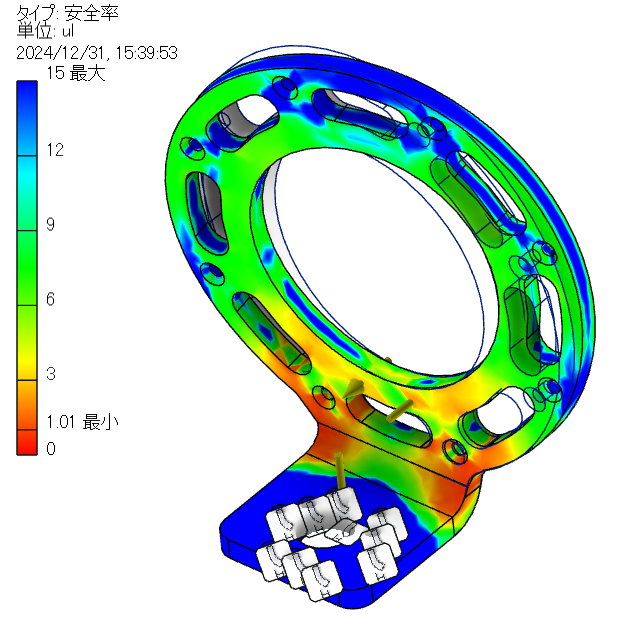
\includegraphics[width=6cm]{images/design/T5.png}
  \caption{Structural analysis results of Part 1 (thickness changed to 5mm)}
  \label{fig:T5}
\end{figure}

\begin{table}[h]
  \centering
  \caption{Specifications of Part 1 (thickness changed to 5mm)}
  \begin{tabular}{lc}
    \hline
    厚み & 5㎜ \\ 
    質量 & 71.1g \\ 
    安全率 & 1.01 \\ \hline
  \end{tabular}
  \label{tab:part1_spec_T5}
\end{table}
\clearpage

次に,板厚を変更せず,形状の改良を行った場合の解析結果を図\ref{fig:T3_80}に示し,設計仕様を表\ref{tab:part1_spec_T3_80}にまとめた.具体的には,図\ref{fig:T3_40}の解析結果を基に,特に強度が不足していると判明した曲げ加工部分の幅を広げる設計変更を行った.

解析の結果,安全率が基準を満たし,十分な強度を確保できることが確認された.また,重量は61.8gであり,板厚を変更した場合(表\ref{tab:part1_spec_T5}参照)と比較して軽量化を実現した.

以上の解析結果を踏まえ,図\ref{fig:shoulder}の部品1について,曲げ加工部分の幅を広げた設計変更を最終設計として採用した.

\begin{figure}[h]
  \centering
  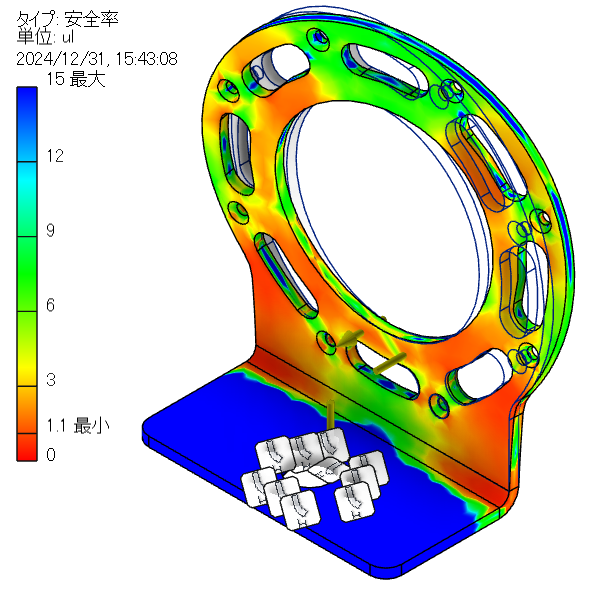
\includegraphics[width=6cm]{images/design/T3_80.png}
  \caption{Structural analysis results of Part 1 (shape optimized)}
  \label{fig:T3_80}
\end{figure}

\begin{table}[h]
  \centering
  \caption{Specifications of Part 1 (shape optimized)}
  \begin{tabular}{lc}
    \hline
    厚み & 3㎜ \\ 
    質量 & 61.8g \\ 
    安全率 & 1.1 \\ \hline
  \end{tabular}
  \label{tab:part1_spec_T3_80}
\end{table}

\subsection{部品2の構造解析}
図\ref{fig:shoulder}の部品2は,アルミフレームを2方向から固定する形状を採用している(図\ref{fig:pitchalumi}参照).最大負荷条件(22Nm)の下で構造解析を実施した結果を図\ref{fig:pitch}に示す.現行の設計では,安全率が0.47と低く,特に赤色で示された箇所において強度不足が確認された.

\begin{figure}[h]
  \centering
  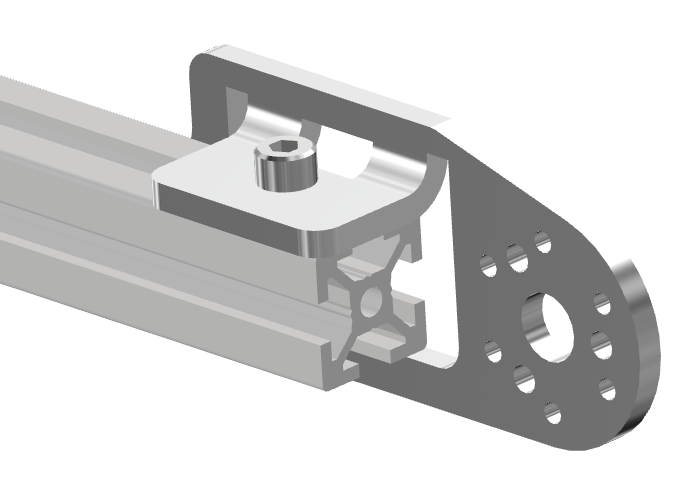
\includegraphics[width=6cm]{images/design/pitchlink.png}
  \caption{Fixing the aluminum frame and part 2}
  \label{fig:pitchalumi}
\end{figure}

\begin{figure}[h]
  \centering
  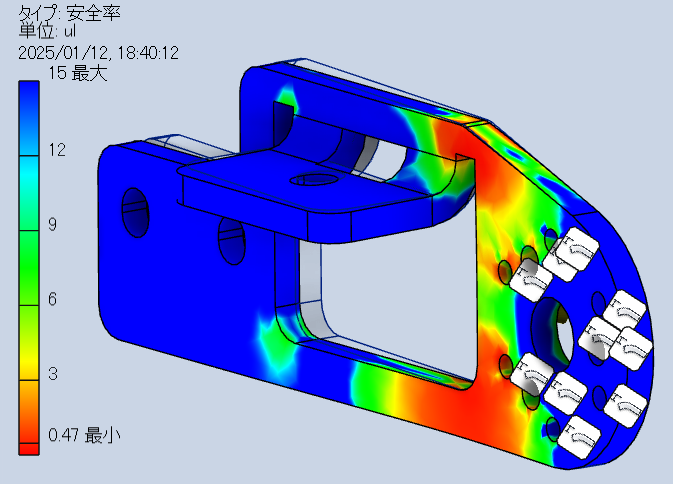
\includegraphics[width=6cm]{images/design/pitch.png}
  \caption{Structural analysis results of Part 2 at maximum output of 22Nm}
  \label{fig:pitch}
\end{figure}

部品の厚みを5mmに変更した場合,安全率は0.58に改善したものの,依然として基準に満たなかった.このため,定格出力(7.5Nm)の条件下で再解析を実施した.解析結果を図\ref{fig:pitchok}に示し,設計仕様を表\ref{tab:part2_spec}にまとめた.この結果,定格条件下では安全率が基準を満たし,十分な強度を確保できることが確認された.

以上より,現設計において部品2の形状変更は行わないこととし,最大出力時の安全率の確保を今後の課題とする.
\begin{figure}[h]
  \centering
  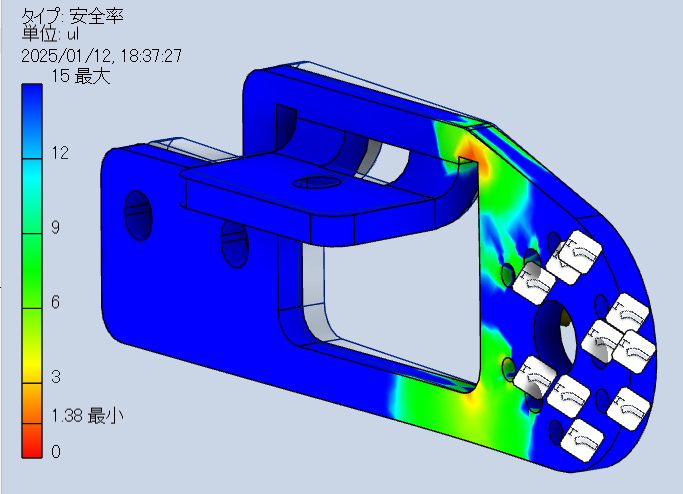
\includegraphics[width=6cm]{images/design/pitchok.png}
  \caption{Structural analysis results of Part 2 at rated output 7.5Nm}
  \label{fig:pitchok}
\end{figure}
\begin{table}[h]
  \centering
  \caption{Specifications of Part 2}
  \begin{tabular}{lc}
    \hline
    厚み & 5㎜ \\ 
    質量 & 34.0g \\ 
    安全率 & 1.38 \\ \hline
  \end{tabular}
  \label{tab:part2_spec}
\end{table}

\newpage
%!TEX root = ../thesis.tex
\section{平行グリッパの設計}
本研究では,リニアガイドとラック&ピニオン機構を用いた平行グリッパを設計した.図\ref{fig:hand}は平行グリッパの分解図である.グリッパの開閉には,QDDモータ(Steadywin GIM3505-8)を使用し,モータに取り付けたギアを介してラック&ピニオン機構で駆動する.グリッパのスライド部分にはリニアガイドを採用している.また,黄色の部品は3Dプリンタでの製作を行う.
\begin{figure}[htbp]
  \centering
  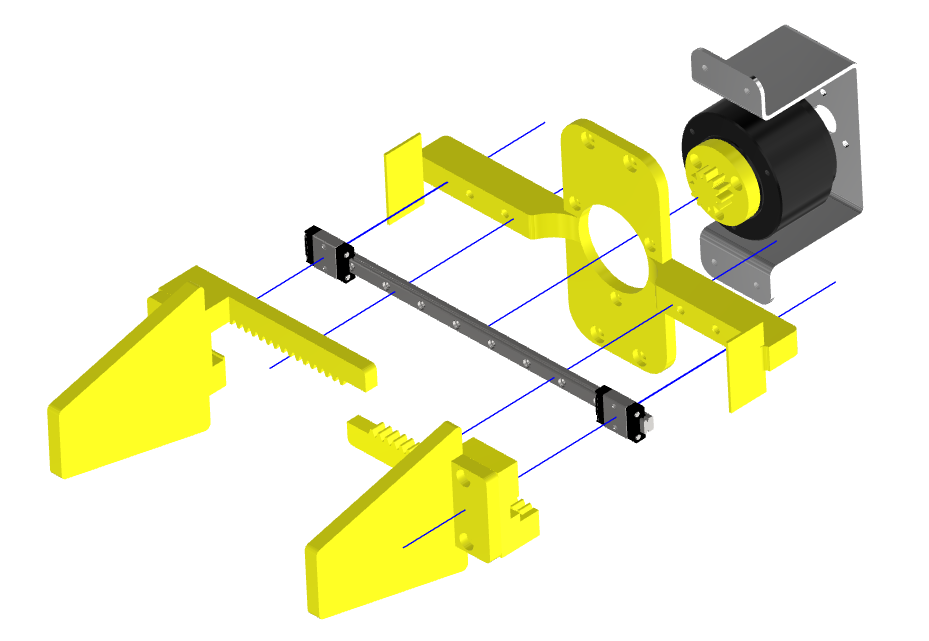
\includegraphics[width=10cm]{images/design/hand.png}
  \caption{Exploded view of parallel gripper}
  \label{fig:hand}
\end{figure}

\newpage
%
%
%% Main Matter
\mainmatter{}
%
\chapter{序論}
\label{chap:introduction}
%
%\input{introduction/preface}
%
%!TEX root = ../thesis.tex

\section{背景}
近年,人手不足を背景にサービスロボットの需要が高まり,日常生活の中で目にする機会が増えている.現在,実用化に至っているサービスロボットは,館内の案内\cite{AYUDA:online},警備\cite{SQ-2:online},掃除\cite{KLEENBOT:online},配膳\cite{BellaBot:online},など,1つの作業に特化したロボットだが,複数作業が行える汎用サービスロボットであるモバイルマニピュレータロボットの開発が進められている.モバイルマニピュレータロボットは,自律移動ロボットにマニピュレータを搭載したロボットで,PAL Robotics社のTIAGo(図\ref{fig:TIAGo}参照) やトヨタ自動車のHSR(図\ref{fig:HSR}参照) などがある.これらのロボットは人に代わって様々な作業ができる汎用的なサービスロボットとして実用化が期待されている\cite{古賀達也201937_707}.本研究では,オフィス環境で活動するモバイルマニピュレータをオフィスロボットと定義して,話を進める.

オフィスロボットは様々な企業や研究室で開発が進められているが,設計データを公開しているものが少なく,標準的なプラットフォームが不足している.ロボットのオープンプラットフォームは,利用者によるハードウェアの改良などが容易にできるだけでなく,技術促進の場としても優れている.例えば,自律移動ロボットのオープンソースハードウェアであるi-Cartシリーズは,本研究室で開発されているorne-boxを始めとした様々なロボットのベースとして活用されている.ハードウェアプラットフォームがあると,ハードウェアを開発する手間が省け,ソフトウェア開発に注力できる.様々な開発者の知識や成果を共有し,技術の発展を加速させることに寄与すると考え,本研究ではオープンプラットフォームオフィスロボットの開発を行う.本項では,オフィスロボットのアームに着目し,設計と製作を行う.

\begin{figure}[h]
  \centering
  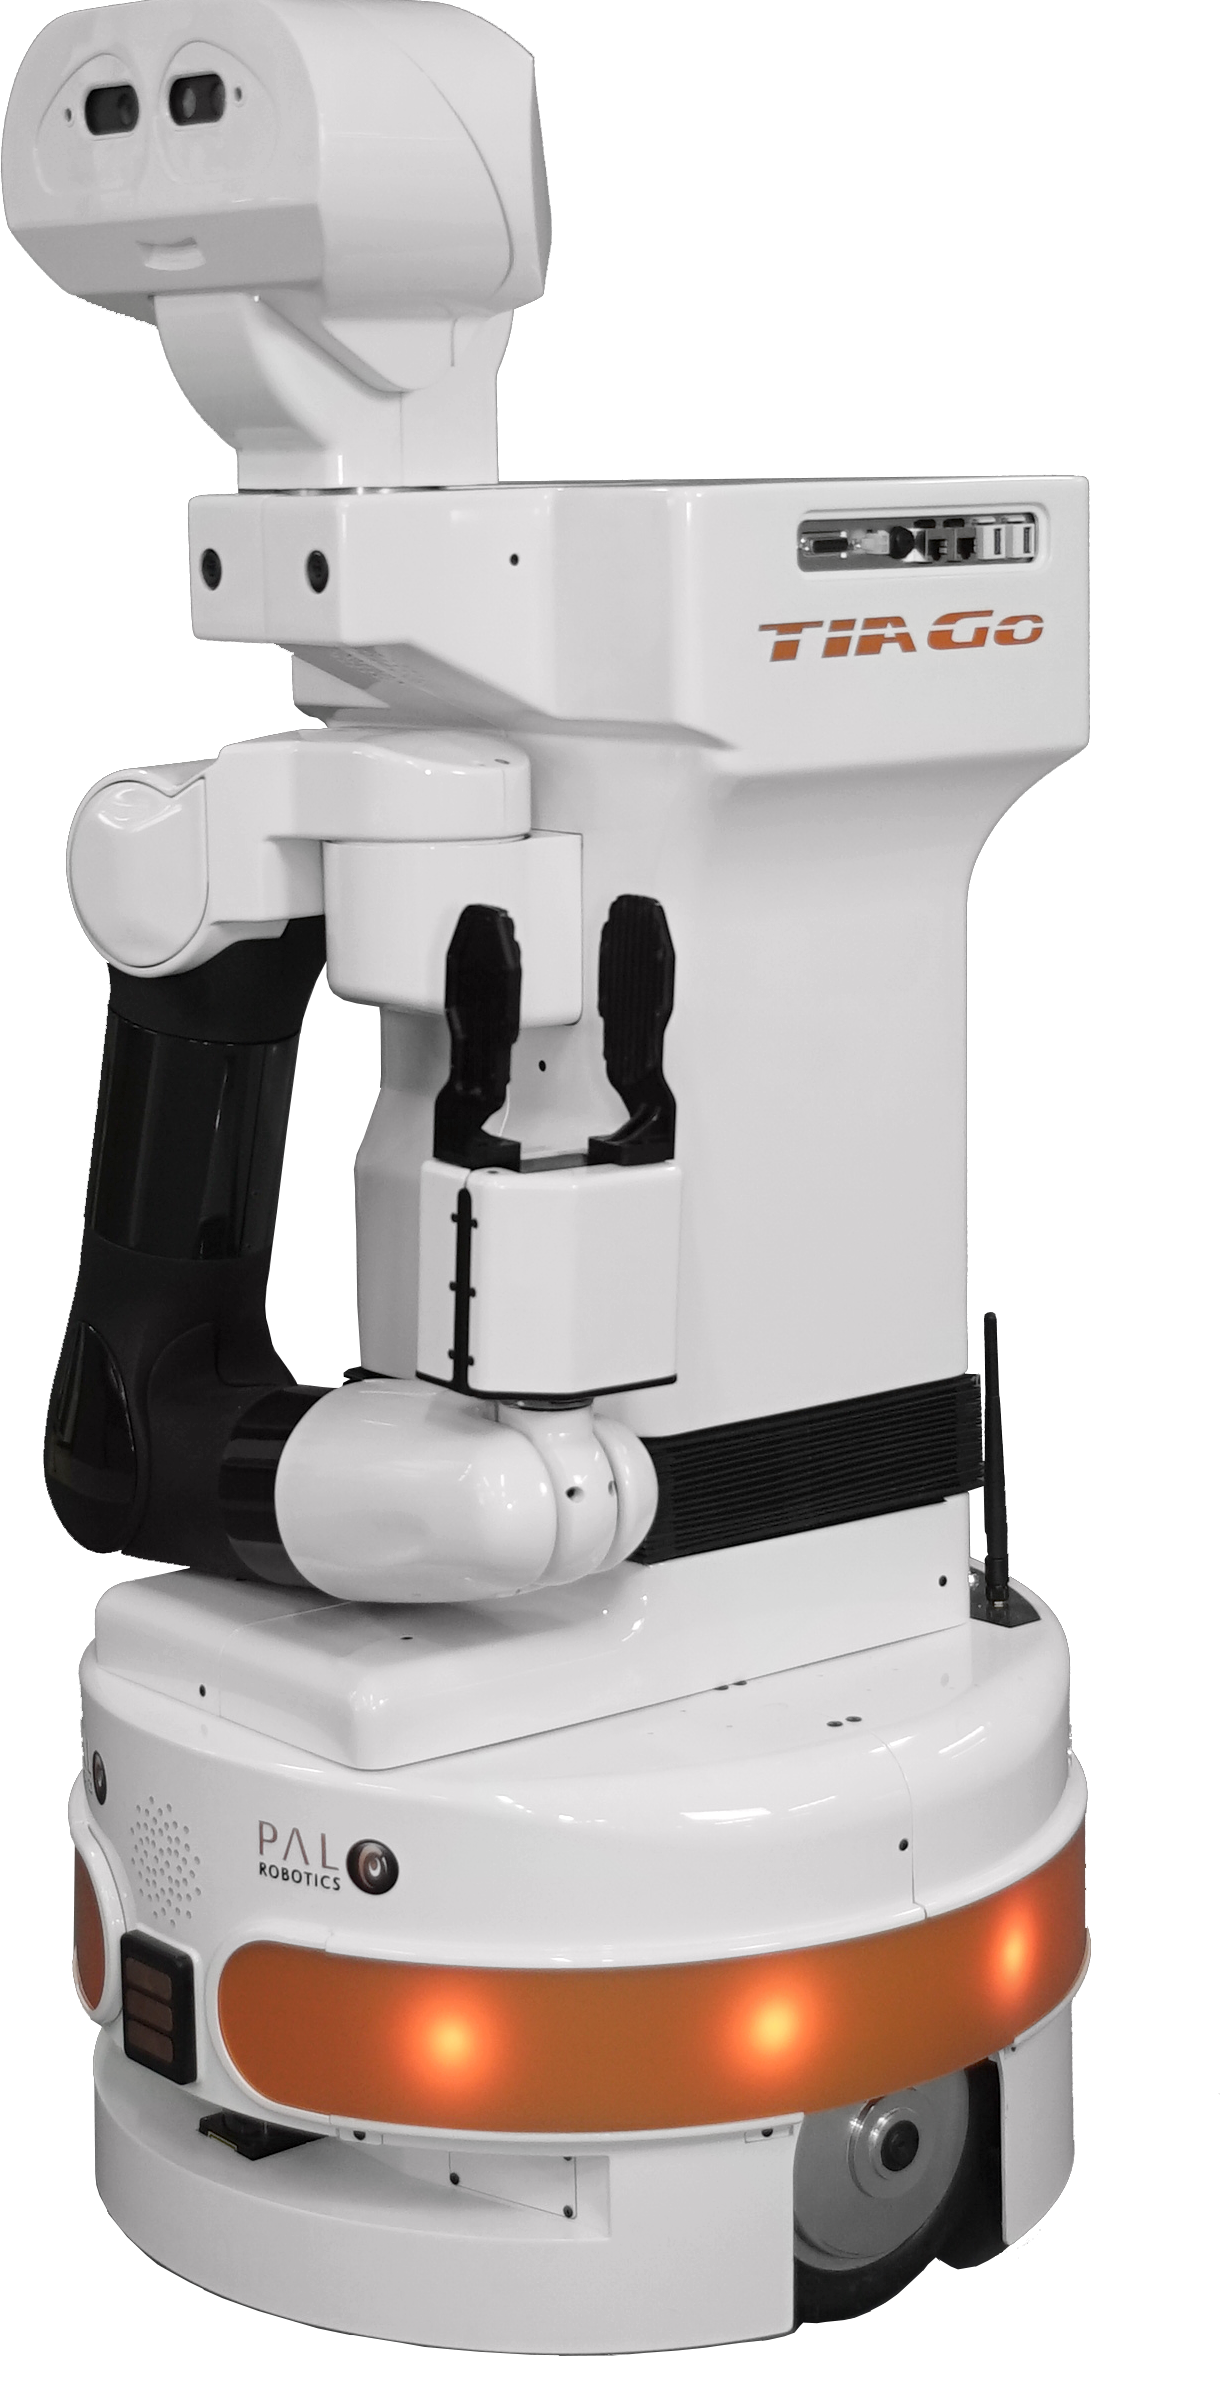
\includegraphics[width=25mm]{images/png/TIAGo.png}
  \caption{TIAGo from PAL-Robotics (source: \cite{TIAGo:online})}
  \label{fig:TIAGo}
\end{figure}
\begin{figure}[h]
  \centering
  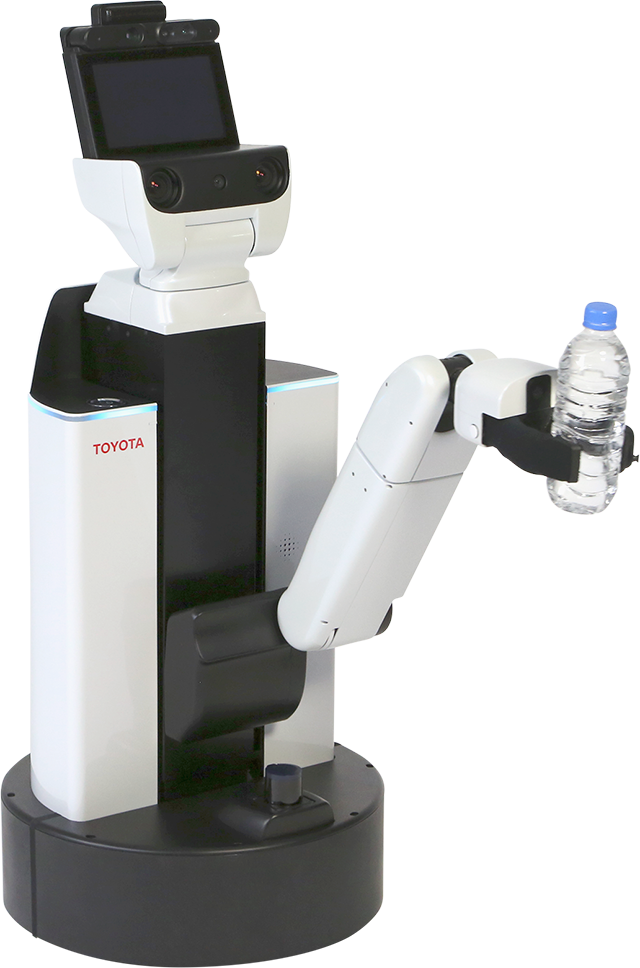
\includegraphics[width=25mm]{images/png/HSR.png}
  \caption{HSR from TOYOTA (source: \cite{HSR:online})}
  \label{fig:HSR}
\end{figure}

\newpage
%!TEX root = ../thesis.tex

\section{QDDモータの採用}
オフィス環境においてロボットアームが人や物に被害を与えないことは極めて重要である.本研究では安全性の向上を目的として,QDD(Quasi Direct Drive)モータを採用する.QDD モータは,低減速比で高いバックドライバビリティを有し,優れた応答性を示す点が特徴である.この特徴により,動作中の予期せぬ接触が発生しても関節が柔軟に動作しやすく,安全性の向上が期待される.

QDDモータに関する研究として,飯塚ら\cite{飯塚浩太2021}は,DDモータに10:1の減速機構を組み合わせたQDDモータを用いた柔軟な3自由度ロボットアーム(図\ref{fig:3DofArm}参照)を開発し,その評価実験を行っている.同研究では,制御周波数を高めることで制御ゲインを向上させることを確認しており,柔軟性と剛性の切り替えが自在に行えることを示している.

また,Gealyら\cite{gealy2019}が開発したBlue(図\ref{fig:blue}参照)では,アームの関節にQDDモータを採用することで,高いバックドライバビリティと応答性を活かした作業を可能にしている.特に,動作中に人間が接触した場合でも,関節が柔軟に動作する特性や,人間が遠隔操作を行い,コーヒーメーカを操作や,机拭き作業などを行えることを示している\cite{Blue:online}.

さらに,Zhaoら\cite{10106520}は,モバイルプラットフォームへの搭載を視野に入れた軽量ロボットアームを開発している(図\ref{fig:qddarm}参照).同アームは6自由度や7自由度のロボットアームが多い中,5自由度で構成されており,部品の形状,素材によって軽量化を図っている.同アームはピックアンドプレースタスクを想定した実験により,高い柔軟性と安全性を実証している.

これらの研究から,QDDモータを適切に制御することで,衝突時の衝撃を軽減し,安全性を向上させることが確認されている.一方で,使用されているQDDモータは,DDモータと低減速比ギアを組み合わせたケースが大半であり,市販のQDDモータをロボットアームに活用した事例は少ない.そのため,市販のQDDモータの技術的なノウハウや応用可能性については,まだ十分に探求されていないのが現状である.

\begin{figure}[h]
  \centering
  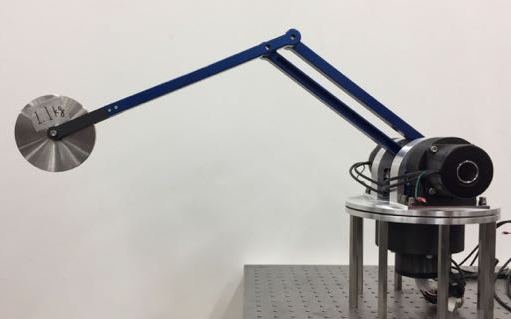
\includegraphics[width=10cm]{images/haikei/3DofArm.png}
  \caption{The Blue robot using QDD motor. (source: \cite{飯塚浩太2021})}
  \label{fig:3DofArm}
\end{figure}
\begin{figure}[h]
  \centering
  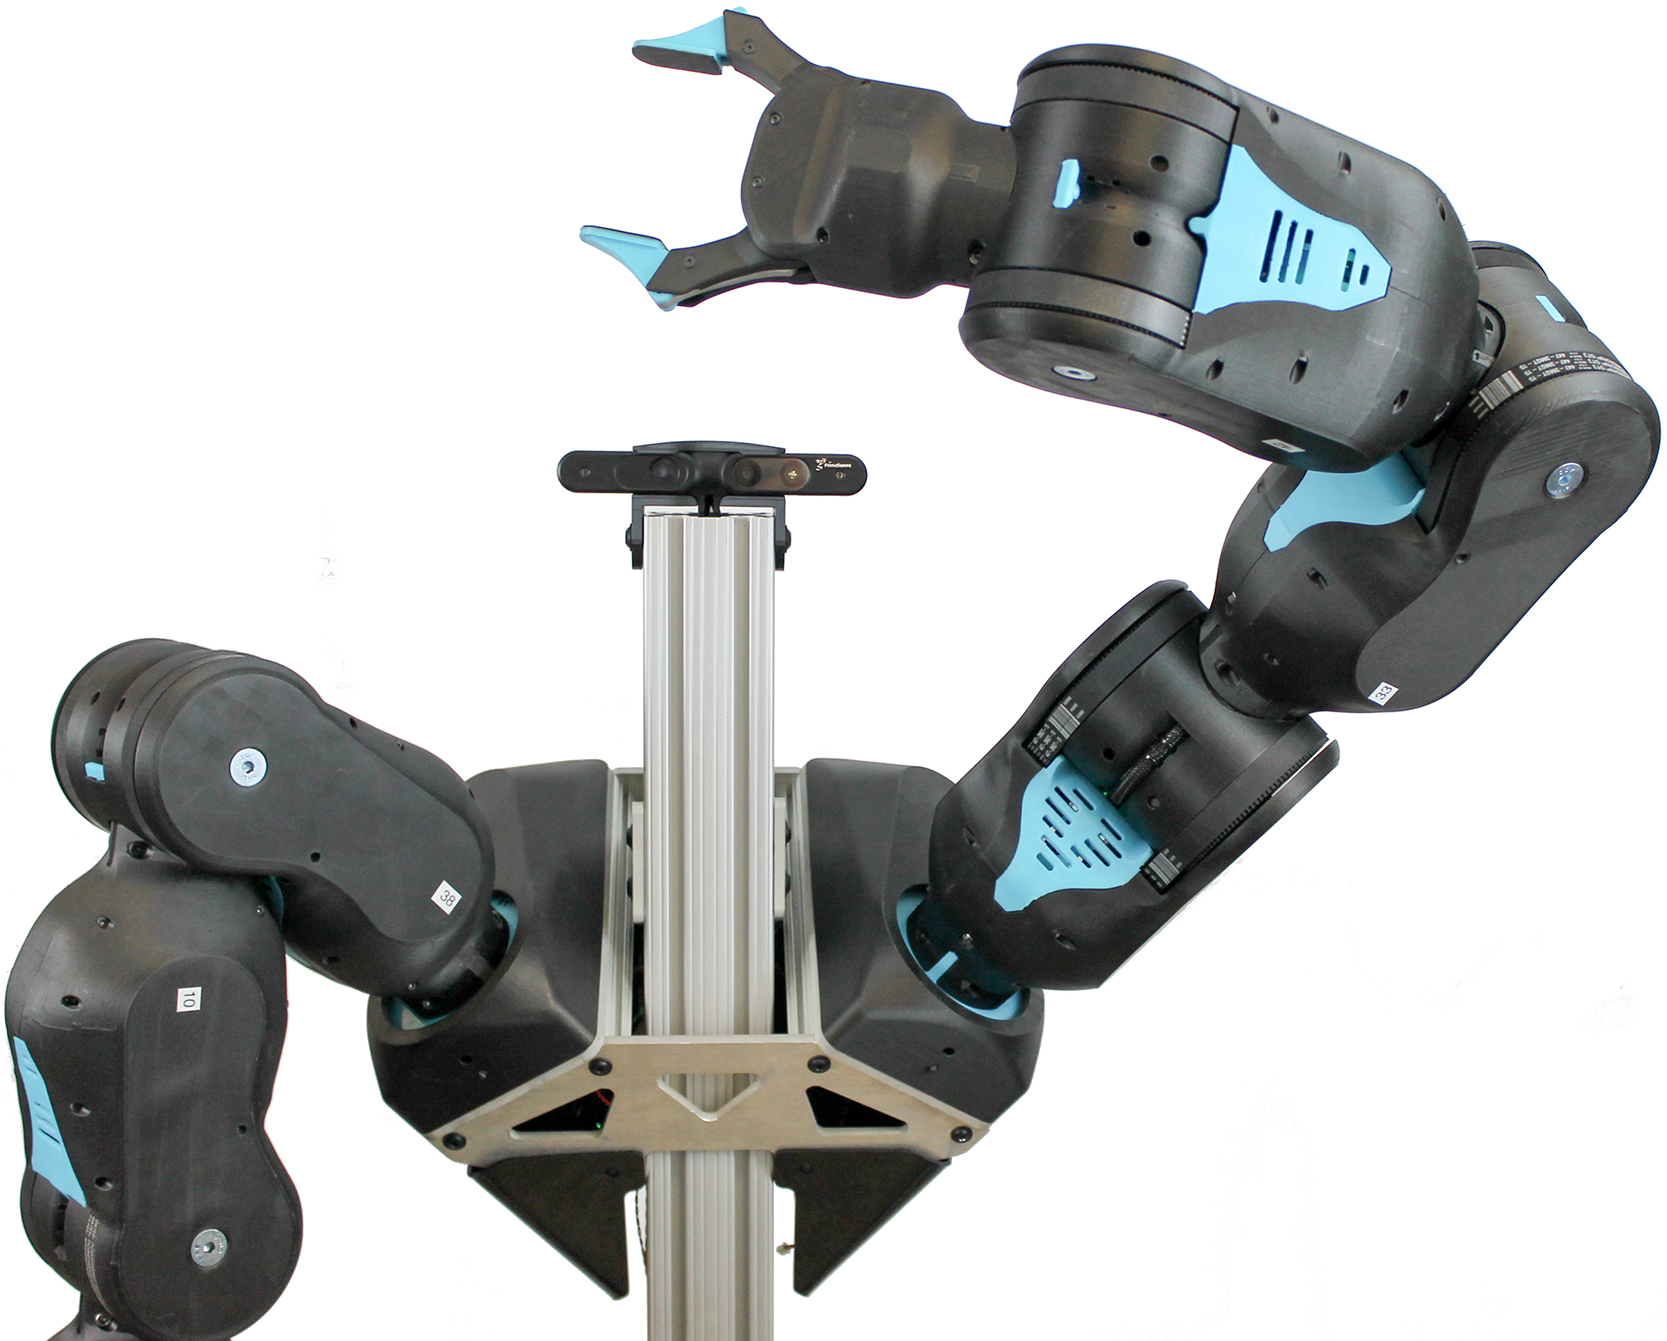
\includegraphics[width=10cm]{images/haikei/twoArmTeaser.jpg}
  \caption{The Blue robot using QDD motor. (source: \cite{Blue:online})}
  \label{fig:blue}
\end{figure}
\begin{figure}[h]
  \centering
  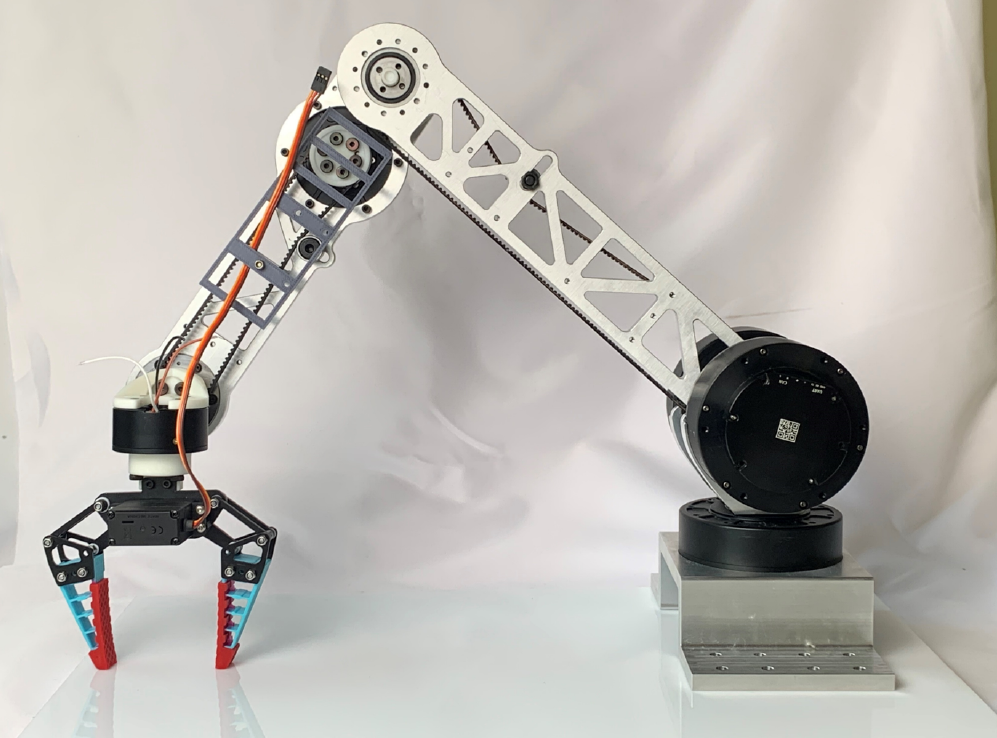
\includegraphics[width=10cm]{images/haikei/qddarm.png}
  \caption{The proposed 5-DOF articulated quasi-direct drive (QDD) robot arm,
  together with a commercial 1-DOF soft gripper. (source: \cite{10106520})}
  \label{fig:qddarm}
\end{figure}
\clearpage
%!TEX root = ../thesis.tex

\section{目的}
本研究は,オープンプラットフォームオフィスロボット開発の第一段階として,応用事例の少ない市販のQDDモータを用いたロボットアームのメカニズムを開発し,その設計データを公開することを目的とする.
\section{本論文の構成}
第1章は,研究背景や目的について述べ,本研究と関連する先行研究や文献について調査して,研究の位置づけを明らかにした.第2章では,オフィスロボットの作業要件とロボットアームの仕様について述べる.第3章では,QDDモータを用いたロボットアームの設計について述べる.第4章では製作について述べる.最後に,第5章で結論と今後の展望を述べる.

\newpage

%

\chapter{設計指針}
\label{chap:second}
%
% %!TEX root = ../thesis.tex
前提として,開発するロボットアームは,オフィスロボットとして適している必要がある.オフィスロボットとして適した仕様を決定するにあたり,本研究では以下の手順を踏んだ.
\begin{enumerate}
  \item 既存オフィスロボットが対象としている作業の調査
  \item 行う作業の決定
  \item 既存オフィスロボットのロボットアームのメカニズム調査
  \item 仕様の決定
\end{enumerate}
まず,「調査した全てのオフィスロボットが行える作業」を基準に作業を決定し,その作業から求められる項目を,ロボットアーム調査の結果を踏まえて整理した.本章では,本研究で対象とする作業の決定過程と,要求仕様の決定について述べる.

\section{作業調査}
開発するロボットアームが対象とする作業を決定するため,既存のオフィスロボットが対象としている作業を調査した.動画や文献をから合計77件の作業事例を抽出したところ,約61\%が台車移動とピック\&プレイスを組み合わせた作業であった.これは,部屋の片づけや荷物の運搬などが代表例である.それ他の作業としては,ドアの開閉,ボタンの押下,フロアの巡回,などが挙げられた.以上の結果から,現在オフィスロボットが対象としている作業の多くは,物体を把持して移動させる作業であると考えられる.本研究で開発するロボットアームは,将来的にオフィスロボットの標準プラットフォームとして活用されることを目指している.その第一歩として,本研究では「机の片づけ作業」を対象とした.

\section{机の片づけ作業}
ここでは,「机の片づけ作業」の詳細を述べる.机の片づけ作業は,机の上に散らばっている物体を事前に設置した箱の中へ移動させる作業である.以下に,具体的に使用する物体の種類や重量,設置位置について以下に述べる.
\subsection{机の上に置く物体}
机の上に置く物体,すなわちロボットが把持対象とする物体は,既存のオフィスロボットが頻繁に把持していた対象を調査したうえで設定した.図\ref{fig:handget}に示すように,最も多かったのは服やタオルなどの衣類で,次にペットボトルや缶ジュースなどの筒状物,お菓子の箱や 200ml 程度のパックジュースなどの箱状物,さらにペンなどの棒状物や雑誌などの薄型物が続いた.以上の結果に基づき,本研究では作業対象としてタオル,缶ジュース,パックジュースの 3 種類を採用する.
\begin{figure}[h]
  \centering
  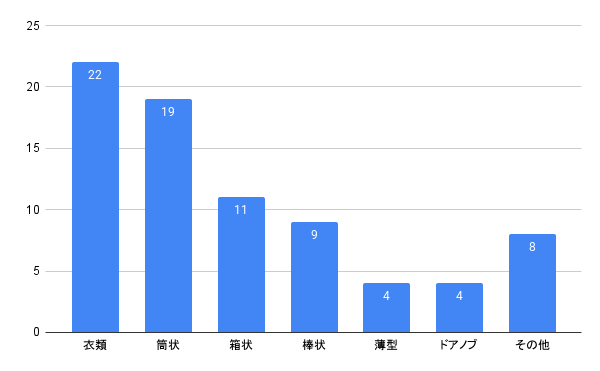
\includegraphics[width=10cm]{images/2syou/handget.png}
  \caption{Survey results of objects grasped by office robots}
  \label{fig:handget}
\end{figure}
\clearpage
\subsection{物体の重量}
調査の中では,人が片手で持てないサイズや重量の大きい物体を扱う事例は見られなかった.そこで,把持対象物の重量は 500g 以下と設定した.
\subsection{物体の設置位置}
次節で詳述するように,既存のオフィスロボットのアームリーチで最小の値は,Hello Robot 社が開発している Stretch 3 の約 0.51m であった.したがって,把持対象物と箱の設置位置は,机の縁から0.5m以内の範囲に設置することとする.
\newpage
% %!TEX root = ../thesis.tex
\section{要求仕様}
前項で設定した作業を基に、要求仕様を決定する.以下に要求仕様とその理由を示す.
\begin{itemize}
  \item アームリーチ70cm程度
  \item 軽量化
  \item 肩2軸(ヨー、ピッチ)、肘1軸(ロール)、手首3軸(ヨー、ピッチ、ロール)の6自由度
  \item 可搬重量500g以上
  \item 平行グリッパ
  \item 
\end{itemize}
\subsection{アームのサイズ}
ロボットアームのサイズは、オフィス環境で活動するのに適したサイズが好ましい。既存のオフィスロボットのアームリーチは、平均約70cm程度である。また、前項で設定した作業より、対象物の設置位置と箱の設置位置は50cm以内の位置であるため、アームリーチ70cm程度あれば作業の遂行も可能であるため望ましい。
\subsection{アーム重量}
アームの重量は、将来的に台車ロボットに搭載することや、双腕ロボットにすることを考えると、軽量であることが望ましい。
\subsection{アームの自由度}
自由度の決定は既存のオフィスロボットを参考に行う。既存のオフィスロボットの自由度を調査した結果を示す。7自由度と6自由度のロボットがほとんどである。6自由度に比べ7自由度は柔軟な操作が可能であるが、アーム重量が増加し、コストも高くなる。そのため、6自由度のアームが望ましい。この際、軸配置についても既存のロボットアームを参考に、肩2軸(ヨー、ピッチ)、肘1軸(ロール)、手首3軸(ヨー、ピッチ、ロール)とする。

\begin{figure}[h]
  \centering
  \includegraphics[width=10cm]{images/armDof.pdf}
  \caption{既存のオフィスロボットの自由度}
  \label{fig:armDof}
\end{figure}

\subsection{可搬重量}
設定した作業では、500g以下の対象物を把持する。そのため、アームの可搬重量は500g以上であることが望ましい。
\subsection{エンドエフェクタ}
既存のオフィスロボットのエンドエフェクタは、Mobile ALOHAに搭載されているロボットアーム(\ref{fig:alohaarm}に示す)のような平行グリッパが多く、様々な形状の物体を把持していることが確認できた。そのため、本研究で開発するアームにも平行グリッパを搭載する。

\begin{figure}[h]
  \centering
  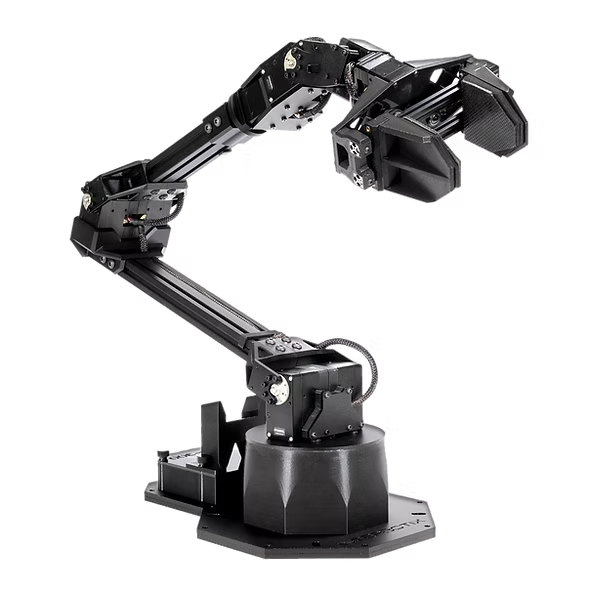
\includegraphics[width=10cm]{images/alohaarm.png}
  \caption{Mobile ALOHO Arm}
  \label{fig:alohaarm}
\end{figure}

\newpage
%!TEX root = ../thesis.tex
本研究で開発するロボットアームは,オープンプラットフォームとしての利用のしやすさを考慮し,オフィスロボットとして最低限の機能を要求する.本章では,従来のオフィスロボットのロボットアーム調査を行い,要求仕様をまとめる.加えて,開発したロボットアームを検証する際に行う作業について,オフィスロボットが対象としている作業を基に検討する.
\section{ロボットアーム調査}
本節では,従来のオフィスロボットのロボットアーム20台を対象に調査し,以下の項目について仕様をまとめる.
\begin{itemize}
  \item アームリーチ
  \item 可搬重量
  \item 自由度
  \item エンドエフェクタ
\end{itemize}
以下では,これらの項目の詳細について述べる.

\subsection{アームリーチ}
従来のオフィスロボットのアームリーチ調査の結果(図\ref{fig:reach}参照),最小値は0.51m,最大値は0.90m,平均値および中央値はいずれも0.71mであった.この結果より,オフィス環境での作業では最低0.51m以上のアームリーチが必要であるといえるが,0.6m以下のロボットが2台であることから,対応できない作業があると想定される.また,アームリーチ0.8mを超えるロボットも10台中2台であり,このことから,0.8mを超えたアームリーチは,現在のオフィスロボットが対象としている作業には過剰であると考えられる.

以上を踏まえ,本研究ではアームリーチの要件を0.6mから0.8mの範囲に設定する.この範囲内のアームリーチであれば,基本的な作業に対応できると考えられる.
\begin{figure}[h]
  \centering
  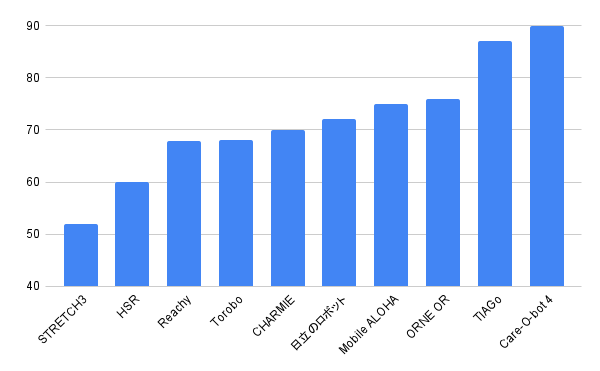
\includegraphics[width=10cm]{images/2syou/reach.png}
  \caption{Office robot arm reach survey results}
  \label{fig:reach}
\end{figure}

\subsection{可搬重量}
従来のオフィスロボットの可搬重量の最小は0.35kgであった(図\ref{fig:payload}参照).よって,現時点のオフィス作業においては0.5kg以上の可搬重量を確保できれば十分であると考えられるため,本研究では0.5kg以上を可搬重量の要件とした.
\begin{figure}
  \centering
  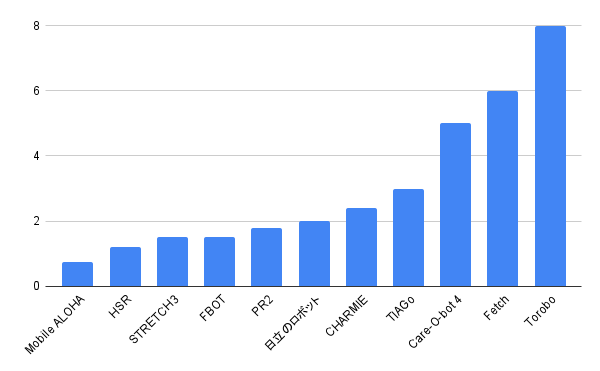
\includegraphics[width=10cm]{images/2syou/payload.png}
  \caption{Office robot payload survey results}
  \label{fig:payload}
\end{figure}
\clearpage

\subsection{自由度}
従来のオフィスロボットのアームの自由度を調査したところ,6自由度と7自由度のロボットが大半であった(\ref{fig:armDof}参照).6自由度の軸配置は,肩2軸(ピッチ,ロール),肘1軸(ロール),手首3軸(ロール,ピッチ,ヨー)で,7自由度ロボットは肩にロール軸が追加されている.7自由度アームは6自由度アームに比べて姿勢の自由度が増す一方で,アーム重量やコストが増加する.本研究ではコスト削減と軽量化を優先し,6自由度を採用した.
\begin{figure}[h]
  \centering
  \includegraphics[width=10cm]{images/2syou/armDof.pdf}
  \caption{Office robot arm DoF survey results}
  \label{fig:armDof}
\end{figure}
\clearpage

\subsection{エンドエフェクタの形状}
従来のオフィスロボットで多く採用されているエンドエフェクタは,TIAGoのような平行グリッパ(図\ref{fig:tiago_hand}参照)である.TIAGoを開発しているPAL Robotics社が公開している動画\cite{TIAGo-movie:online}では,布,ジュース缶,スプレー缶,ジュースパック,板状物など多様な形状の物体を把持している様子が確認できる.本研究においても多様な形状の物体把持が求められるため,平行グリッパを採用した.
\begin{figure}[h]
  \centering
  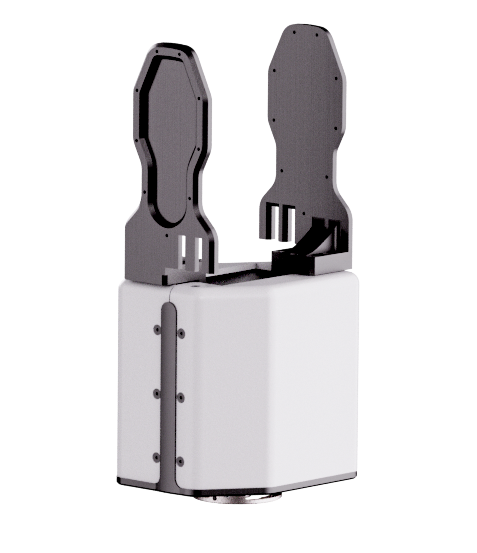
\includegraphics[width=8cm]{images/2syou/tiago_hand.png}
  \caption[End effectior of TIAGo]{End effectior of TIAGo (source: \cite{TIAGo:online})}
  \label{fig:tiago_hand}
\end{figure}
\clearpage

\subsection{オフィスロボットのロボットアームとして要求される項目}
以上を踏まえ,本研究で開発するロボットアームに,以下の項目を要求する.これを仕様として,ロボットアームのメカニズムを設計する.
\begin{itemize}
  \item 0.6m - 0.8mのアームリーチ
  \item 500g以上の可搬重量
  \item 6自由度アーム
  \item 平行グリッパのエンドエフェクタ
\end{itemize}
\newpage
%!TEX root = ../thesis.tex
\section{作業調査}
本研究では,従来のオフィスロボットが対象としている作業を調査し,ロボットアームの検証に適した作業対象を検討する.本研究で開発するロボットアームは,オフィスロボットとして最低限の機能を満たすことを目的としている.そのため,アームの性能を効果的に検証するためには,従来のオフィスロボットが頻繁に対象としており,オフィス環境における基本的な作業として位置づけられるタスクを選定することが重要である.

従来のオフィスロボットが実施している作業事例を動画および文献から収集し,合計77例を抽出した.その結果,約61\%の作業が台車移動とピック\&プレースを組み合わせた作業であることが確認された.代表的な事例として,部屋の片付けや荷物の運搬が挙げられる.その他の作業事例として,ドアの開閉,ボタンの押下,フロアの巡回などが観察された.

これらの結果から,現行のオフィスロボットが主に対象としている作業は,物体を把持し移動させる作業であると推察される.また,ロボットアームの検証作業を選定するにあたっては,基本的な作業であることに加え,多様な物体操作および他の作業への応用性を考慮することが重要である.以上を踏まえ,ロボットアームの検証対象として「机の片付け作業」を選定することが適切であると判断した.

机の片付け作業は,多様な物体の把持能力が求められるだけでなく,研究者が自由に操作条件を設定しやすい特性を有している.さらに,本作業は,散乱した床の片付け作業や棚の物体操作など,他のタスクへの応用が可能であるため,ロボットアームの性能評価において有用性が高いと考える.
\newpage
%
\chapter{設計}
\label{chap:third}
%
本章ではロボットアームのメカニズムの設計について述べる.
まず,選定したQDDモータについて説明し,ロボットアームの設計について述べる.

%!TEX root = ../thesis.tex
\section{オープンプラットフォームを意識した設計}
\newpage
%!TEX root = ../thesis.tex
\section{QDDモータの選定}
飯塚ら\cite{飯塚浩太2021}の研究では,減速比10:1のQDDモータが使用されている.また,Zhaoら\cite{10106520}の研究においては,減速比9:1のQDDモータが採用されていた.これらの先行研究は,ロボットアームと人の衝突時の衝撃力軽減を実現するためには,この程度の減速比を持つモータを採用することが有効であることを示唆している.

さらに,本研究ではオープンプラットフォームの観点を重視し,他のロボットアームに使用されているモータと同程度,またはそれ以下の価格であることを選定基準とした.調査対象としたオフィスロボットのうち,ロボットアームに使用しているアクチュエータの価格は,約3万円から約8万円であったため,価格上限を8万円に設定した.

以上を踏まえ,本研究では,持つSteadywinのGIM8108-8とGIM3505-8を採用した.減速比は8:1であり,先行研究で使用されていたモータと同程度の減速比を持つ.また,価格は約19,000円と約18,000円であり,価格上限である8万円を下回っている.
\subsection{選定したモータの性能}
表\ref{tab:QDDComparison}に,選定したQDDモータとReachy\cite{Reachy:online}のアームに使用されているモータ(Dynamixel MX-106T)の比較を示す.選定したSteadywinのGIM8108-8とGIM3505-8は,減速比が8:1で,先行研究で使用していた減速比と近しい物になっている.適切に制御することで衝突時の衝撃を軽減することが可能である.また,許容ラジアル荷重とアキシアル荷重も高いため,追加の補強部品を必要とせずにロボットアームの構造を簡略化することが可能である.
\begin{table}[]
  \centering
  \caption{QDD motor performance comparison}
  \label{tab:QDDComparison}
  \begin{tabular}{lccc}
  \hline
               & \begin{tabular}[c]{@{}c@{}}SteadyWin\\ GIM8108-8\end{tabular} & \begin{tabular}[c]{@{}c@{}}SteadyWin\\ GIM3505-8\end{tabular} & \begin{tabular}[c]{@{}c@{}}Dynamixel\\ MX-106T\end{tabular} \\ \hline
  減速比          & 8 : 1                                                         & 8 : 1                                                         & 225 : 1                                                     \\
  定格トルク(Nm)    & 7.5                                                           & 0.65                                                          & -                                                           \\
  最大トルク(Nm)    & 22                                                            & 1.27                                                          & 10                                                          \\
  重量(g)        & 396                                                           & 97                                                            & 153                                                         \\
  無負荷回転数(rpm)  & 320                                                           & 384                                                           & 55                                                          \\
  許容ラジアル荷重(N)  & 900                                                           & 300                                                           & 40                                                          \\
  許容アキシアル荷重(N) & 225                                                           & 75                                                            & 20                                                          \\
  価格(円)        & 約19,000                                                       & 約18,000                                                       & 約80,000                                                     \\ \hline
  \end{tabular}
\end{table}

\subsection{QDDモータの欠点}
QDDモータは高トルク・高スピードでの動作が可能であるという利点を持つ一方で、この特性は制御が不十分な場合にリスクとなる.特に、通電時に動作が暴走した場合、一般的なモータと比較して周囲の人や機器への被害が大きい.そのため、QDDモータを安全に運用するためには、適切な制御と安全対策が必要である.
\newpage
%!TEX root = ../thesis.tex
\section{基本的な性能}
設計したロボットアームの基本的な性能を述べる.
\subsection{アームサイズ}
図\ref{fig:link_length}にロボットアームのアームリーチとリンク長を示す.人間の腕の長さの比\cite{humanarm:online}を参考に,肩から肘までは290㎜,肘から手首までは220㎜とした.アームリーチは660㎜であり,要求仕様の700㎜程度を満たしている.図\ref{fig:arm_size}にアームサイズを示す.比較のため,机とボトルを模したものを配置している.

\begin{figure}[htbp]
  \centering
  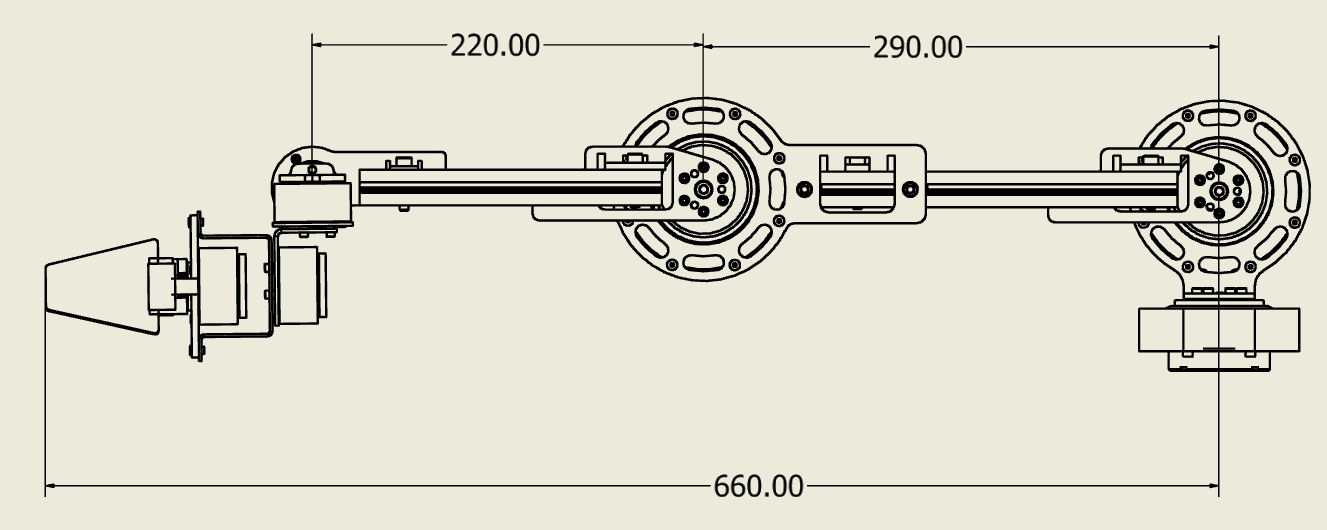
\includegraphics[width=10cm]{images/link_length.png}
  \caption{Arm reach and link length}
  \label{fig:link_length}
\end{figure}

\begin{figure}[htbp]
  \centering
  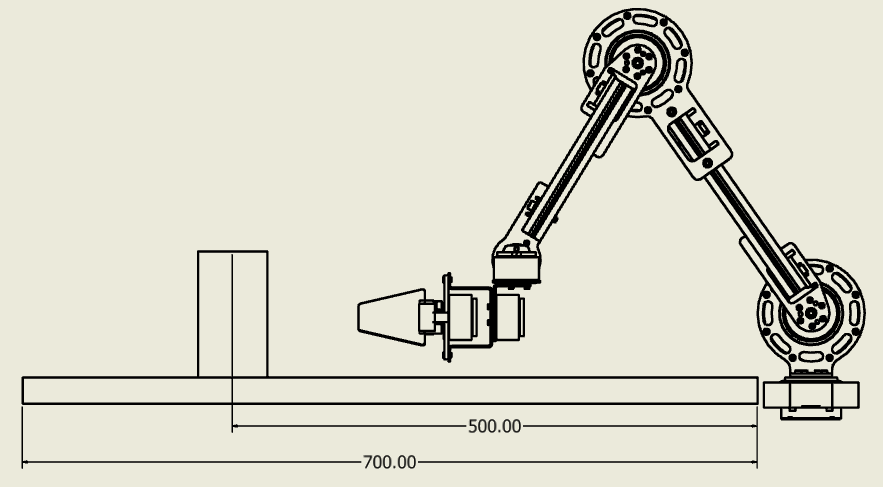
\includegraphics[width=10cm]{images/hikaku.png}
  \caption{Arm size}
  \label{fig:arm_size}
\end{figure}

\clearpage

\subsection{可動範囲}
図\ref{fig:arm_short},図\ref{fig:arm_long}にアームの最小可動範囲と最大可動範囲を示す.最小可動範囲は,アームの部品が干渉することなく動作できる最小の範囲を示しており,最大可動範囲はアームを最大まで伸ばしたときの範囲を示している.

\begin{figure}[htbp]
  \centering
  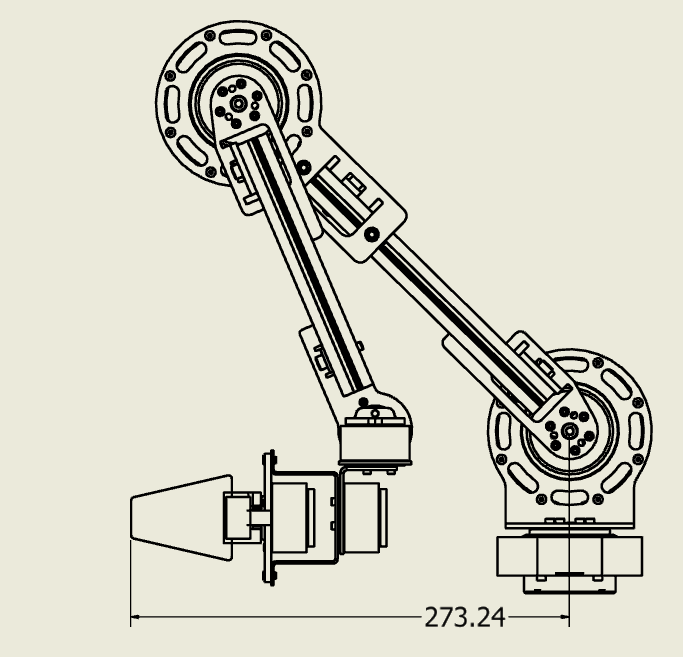
\includegraphics[width=10cm]{images/design/arm_short.png}
  \caption{Minimum range of motion}
  \label{fig:arm_short}
\end{figure}

\begin{figure}[htbp]
  \centering
  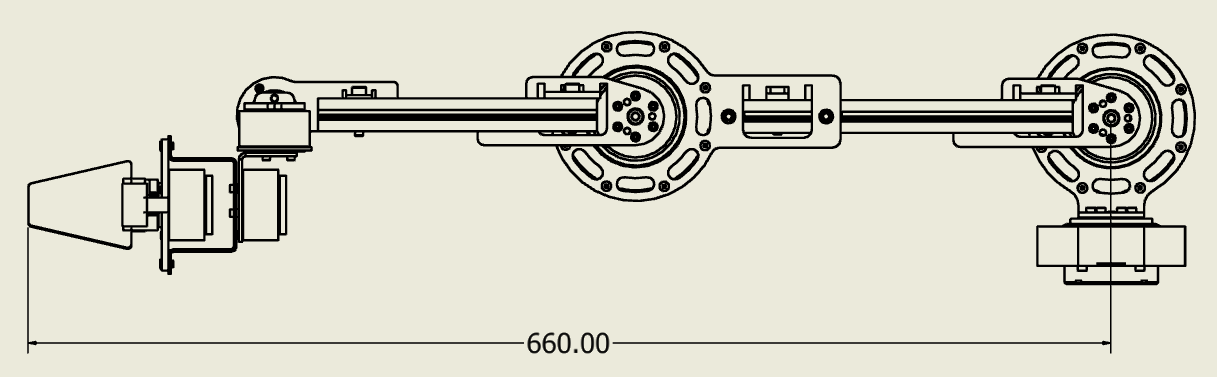
\includegraphics[width=10cm]{images/design/arm_long.png}
  \caption{Minimum range of motion}
  \label{fig:arm_long}
\end{figure}

\subsection{アームの手先の移動}
アームの手先の移動の様子を図\ref{fig:move1},図\ref{fig:move2},図\ref{fig:move3},図\ref{fig:move4}に示す.

\begin{figure}[h]
  \centering
  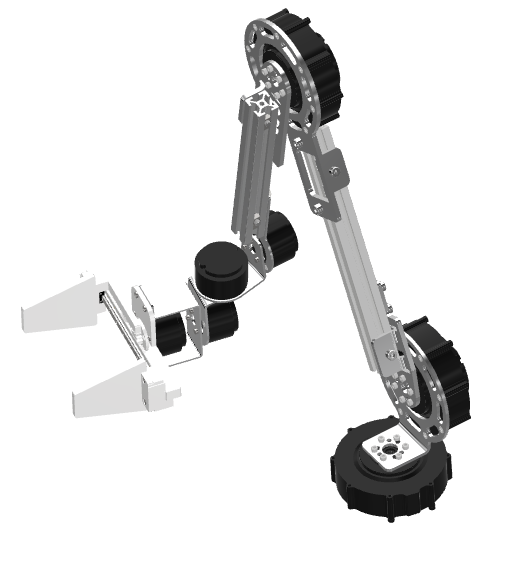
\includegraphics[width=10cm]{images/design/migitika.png}
  \caption{Stretched out to the right}
  \label{fig:move1}
\end{figure}

\begin{figure}[h]
  \centering
  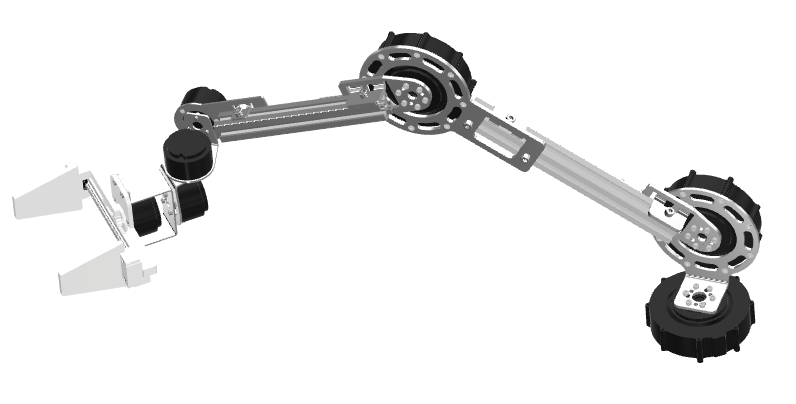
\includegraphics[width=10cm]{images/design/migioku.png}
  \caption{Stretched out to the right}
  \label{fig:move2}
\end{figure}

\begin{figure}[h]
  \centering
  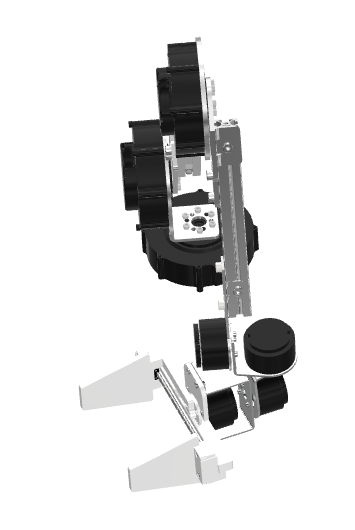
\includegraphics[width=8cm]{images/design/hidaritika.png}
  \caption{Stretched out to the left}
  \label{fig:move3}
\end{figure}

\begin{figure}[h]
  \centering
  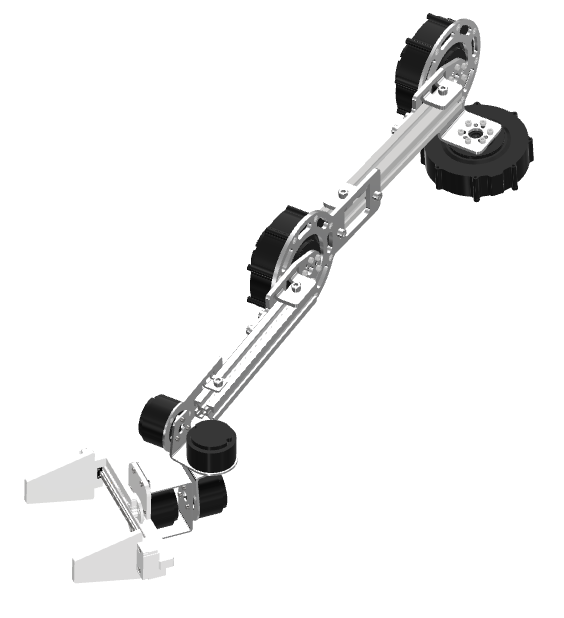
\includegraphics[width=10cm]{images/design/hidarioku.png}
  \caption{Stretched out to the left}
  \label{fig:move4}
\end{figure}
\clearpage

\subsection{可搬重量}
肩ピッチ軸のQDDモータ(SteadyWin GIM8108-8)の定格トルクは7.5Nm,最大トルクは22Nmである.アームを伸ばしたときに自重を支えるために必要なトルクを求め,常時把持することのできる物体の重量と,瞬間的に把持することのできる物体の重量を求める.
\subsubsection{自重を支える為に必要なトルク}
図\ref{fig:CoG}にアームの重心を示す.アームの重心は肩ピッチ軸から0.334mの位置にあり,アームの重さは1.31kgである.重力加速度を9.8m/s$^2$とすると,肩ピッチ軸にかかるトルク$T$は次のように求められる.
\begin{equation}
  T = 1.31 \times 9.8 \times 0.334 = 4.2 Nm
\end{equation}
\begin{figure}[h]
  \centering
  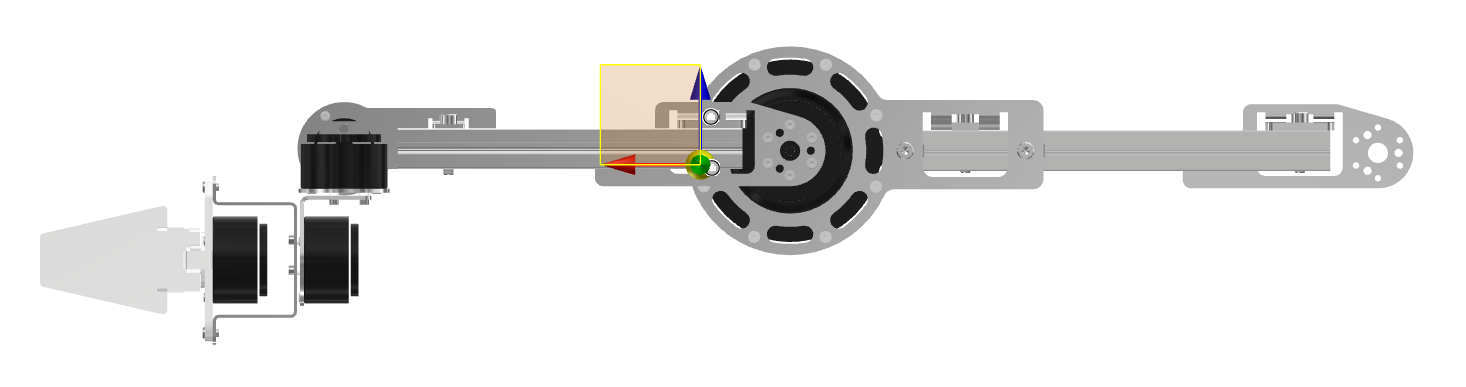
\includegraphics[width=10cm]{images/design/CoG.png}
  \caption{Center of gravity}
  \label{fig:CoG}
\end{figure}

\subsubsection{常時把持することのできる物体の重量}
アームの定格トルクから,自重を支える為に必要なトルクを引くと3.3Nmであり,肩ピッチ軸から手先までの距離は0.66mである.したがって,常時把持することのできる物体の重量$m$は次のように求められる.
\begin{equation}
  m = 3.3 / (9.8 \times 0.66) = 0.51kg
\end{equation}

\subsubsection{瞬間的に把持することのできる物体の重量}
同様に,最大トルクから自重を支える為に必要なトルクを引くと17.8Nmである.したがって,瞬間的に把持することのできる物体の重量$M$は次のように求められる.
\begin{equation}
  m = 17.8 / (9.8 \times 0.66) = 2.75kg
\end{equation}


\clearpage
\newpage
%!TEX root = ../thesis.tex
\section{強度確認}
設計したロボットアームの強度確認のため,Autodesk Inventorの機能である構造解析を行った.解析における安全率が1以上であれば,強度が十分であると判断した.図\ref{fig:shoulder}に肩部の構成を示す.肩部は,ヨー軸モータとピッチ軸モータを繋ぐ図\ref{fig:shoulder}の部品1,およびリンクの一部である,部品2から構成されている.部品1および部品2には,いずれもアルミニウム合金(A5052)を使用している.

本節では,構造解析による部品の強度確認について述べる.

\begin{figure}[h]
  \centering
  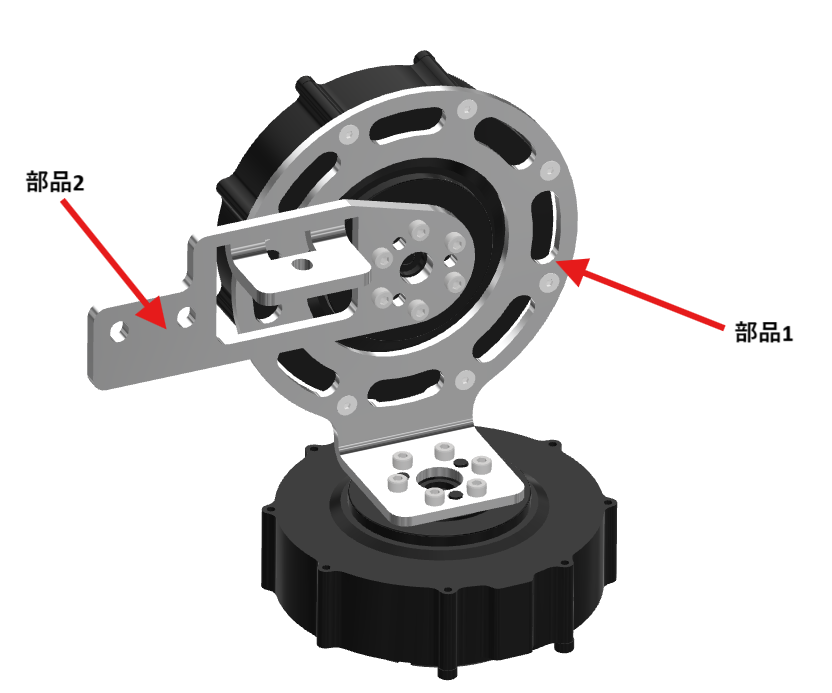
\includegraphics[width=10cm]{images/design/shoulder.png}
  \caption{Configuration of the shoulder components}
  \label{fig:shoulder}
\end{figure}

\subsection{部品1の構造解析}
図\ref{fig:shoulder}の部品1は,ヨー軸モータが最大出力22Nmを発生した際に最大負荷を受ける部品である.図\ref{fig:T3_40}に構造解析結果を示し,設計仕様を表\ref{tab:part1_spec}にまとめた.解析の結果,安全率は0.39であり,強度が不足していることが確認された.特に,図\ref{fig:T3_40}の結果から,曲げ加工部分において強度が不足していることが明らかとなった.この課題を解決するため,「板厚を変更した部品」と「形状を変更した部品」の2つの設計案を検討し,それぞれ再解析を実施した.

\begin{figure}[h]
  \centering
  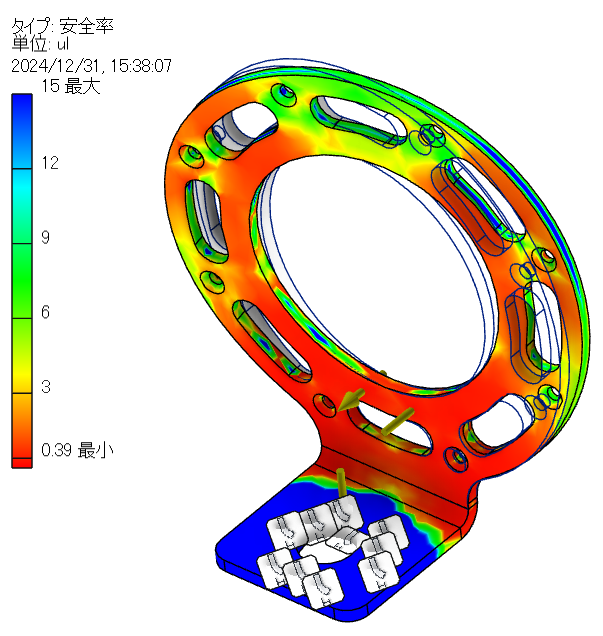
\includegraphics[width=6cm]{images/design/T3_40.png}
  \caption{Structural analysis results of Part 1}
  \label{fig:T3_40}
\end{figure}

\begin{table}[h]
  \centering
  \caption{Specifications of Part 1}
  \begin{tabular}{lc}
    \hline
    厚み & 3㎜ \\ 
    質量 & 43.6g \\ 
    安全率 & 0.39 \\ \hline
  \end{tabular}
  \label{tab:part1_spec}
\end{table}
\clearpage

\subsection{設計の変更}
部品の形状はそのままに,板厚を3mmから5mmに変更した場合の構造解析結果を図\ref{fig:T5}に示し,設計仕様を表\ref{tab:part1_spec_T5}にまとめた.解析の結果,安全率は基準の1を超え,強度が十分であることが確認された.ただし,質量が27.5g増加するという結果が得られた.

\begin{figure}[h]
  \centering
  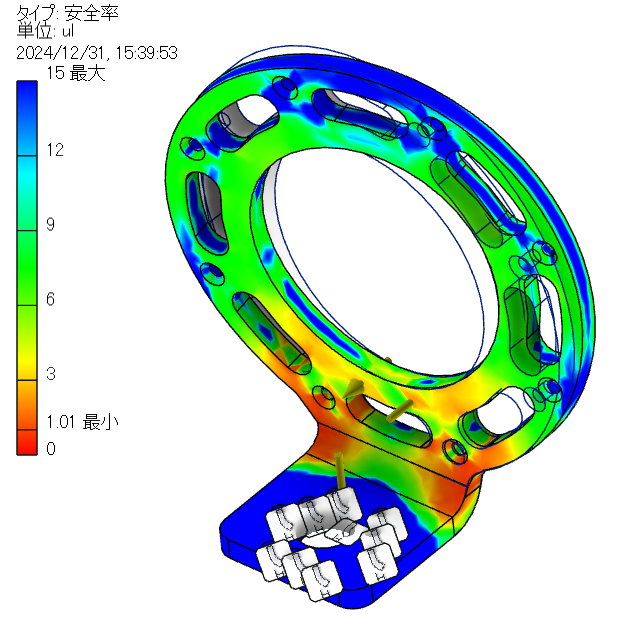
\includegraphics[width=6cm]{images/design/T5.png}
  \caption{Structural analysis results of Part 1 (thickness changed to 5mm)}
  \label{fig:T5}
\end{figure}

\begin{table}[h]
  \centering
  \caption{Specifications of Part 1 (thickness changed to 5mm)}
  \begin{tabular}{lc}
    \hline
    厚み & 5㎜ \\ 
    質量 & 71.1g \\ 
    安全率 & 1.01 \\ \hline
  \end{tabular}
  \label{tab:part1_spec_T5}
\end{table}
\clearpage

次に,板厚を変更せず,形状の改良を行った場合の解析結果を図\ref{fig:T3_80}に示し,設計仕様を表\ref{tab:part1_spec_T3_80}にまとめた.具体的には,図\ref{fig:T3_40}の解析結果を基に,特に強度が不足していると判明した曲げ加工部分の幅を広げる設計変更を行った.

解析の結果,安全率が基準を満たし,十分な強度を確保できることが確認された.また,重量は61.8gであり,板厚を変更した場合(表\ref{tab:part1_spec_T5}参照)と比較して軽量化を実現した.

以上の解析結果を踏まえ,図\ref{fig:shoulder}の部品1について,曲げ加工部分の幅を広げた設計変更を最終設計として採用した.

\begin{figure}[h]
  \centering
  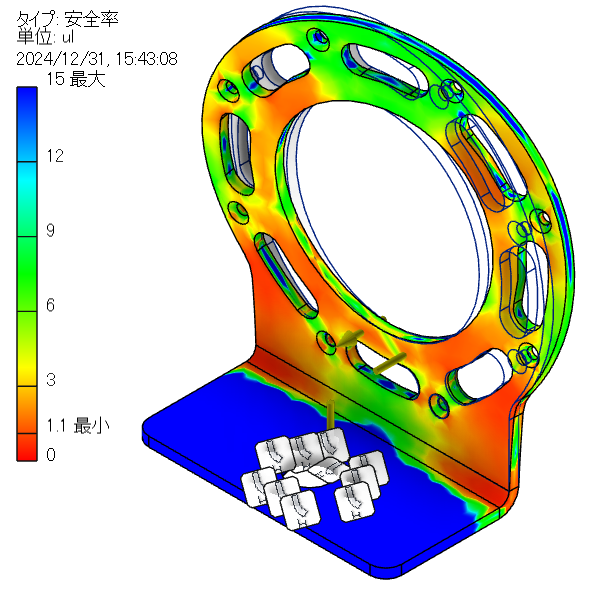
\includegraphics[width=6cm]{images/design/T3_80.png}
  \caption{Structural analysis results of Part 1 (shape optimized)}
  \label{fig:T3_80}
\end{figure}

\begin{table}[h]
  \centering
  \caption{Specifications of Part 1 (shape optimized)}
  \begin{tabular}{lc}
    \hline
    厚み & 3㎜ \\ 
    質量 & 61.8g \\ 
    安全率 & 1.1 \\ \hline
  \end{tabular}
  \label{tab:part1_spec_T3_80}
\end{table}

\subsection{部品2の構造解析}
図\ref{fig:shoulder}の部品2は,アルミフレームを2方向から固定する形状を採用している(図\ref{fig:pitchalumi}参照).最大負荷条件(22Nm)の下で構造解析を実施した結果を図\ref{fig:pitch}に示す.現行の設計では,安全率が0.47と低く,特に赤色で示された箇所において強度不足が確認された.

\begin{figure}[h]
  \centering
  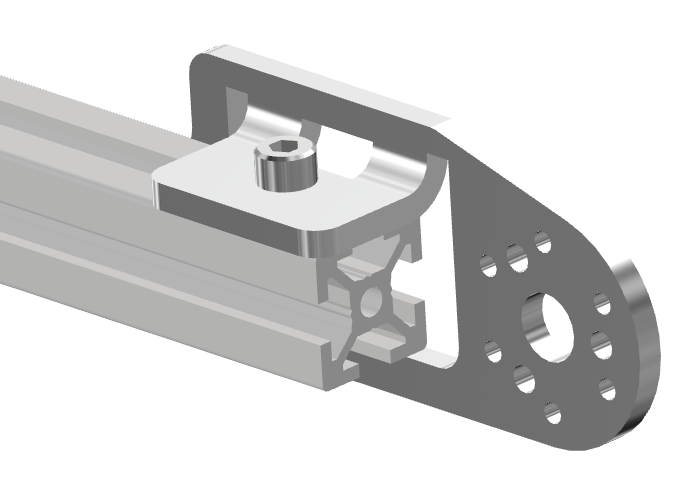
\includegraphics[width=6cm]{images/design/pitchlink.png}
  \caption{Fixing the aluminum frame and part 2}
  \label{fig:pitchalumi}
\end{figure}

\begin{figure}[h]
  \centering
  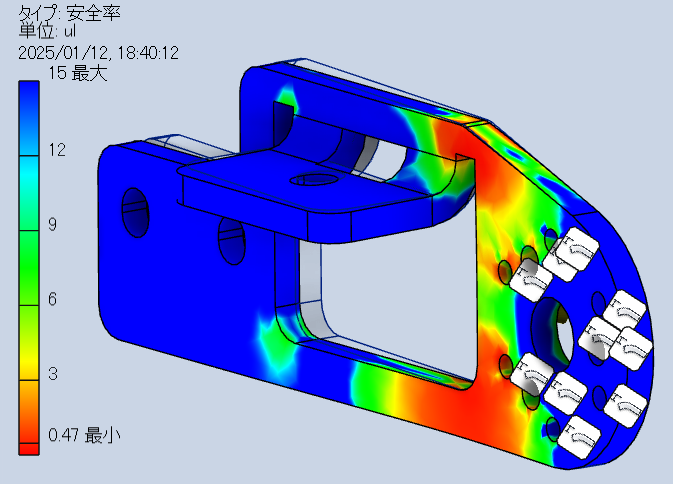
\includegraphics[width=6cm]{images/design/pitch.png}
  \caption{Structural analysis results of Part 2 at maximum output of 22Nm}
  \label{fig:pitch}
\end{figure}

部品の厚みを5mmに変更した場合,安全率は0.58に改善したものの,依然として基準に満たなかった.このため,定格出力(7.5Nm)の条件下で再解析を実施した.解析結果を図\ref{fig:pitchok}に示し,設計仕様を表\ref{tab:part2_spec}にまとめた.この結果,定格条件下では安全率が基準を満たし,十分な強度を確保できることが確認された.

以上より,現設計において部品2の形状変更は行わないこととし,最大出力時の安全率の確保を今後の課題とする.
\begin{figure}[h]
  \centering
  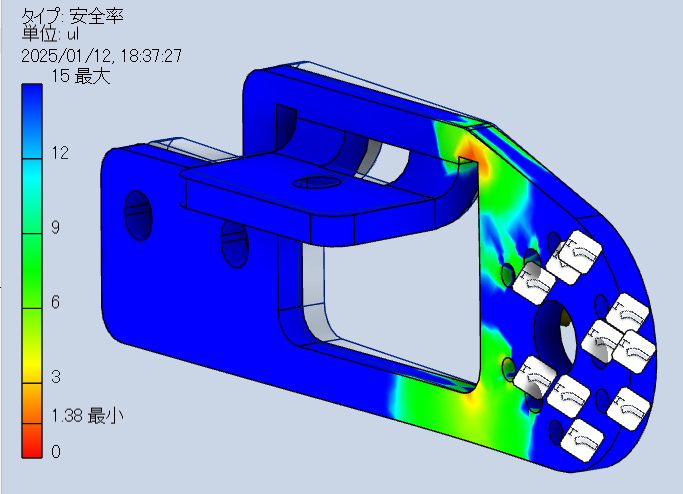
\includegraphics[width=6cm]{images/design/pitchok.png}
  \caption{Structural analysis results of Part 2 at rated output 7.5Nm}
  \label{fig:pitchok}
\end{figure}
\begin{table}[h]
  \centering
  \caption{Specifications of Part 2}
  \begin{tabular}{lc}
    \hline
    厚み & 5㎜ \\ 
    質量 & 34.0g \\ 
    安全率 & 1.38 \\ \hline
  \end{tabular}
  \label{tab:part2_spec}
\end{table}

\newpage
%!TEX root = ../thesis.tex
\section{平行グリッパの設計}
本研究では,リニアガイドとラック&ピニオン機構を用いた平行グリッパを設計した.図\ref{fig:hand}は平行グリッパの分解図である.グリッパの開閉には,QDDモータ(Steadywin GIM3505-8)を使用し,モータに取り付けたギアを介してラック&ピニオン機構で駆動する.グリッパのスライド部分にはリニアガイドを採用している.また,黄色の部品は3Dプリンタでの製作を行う.
\begin{figure}[htbp]
  \centering
  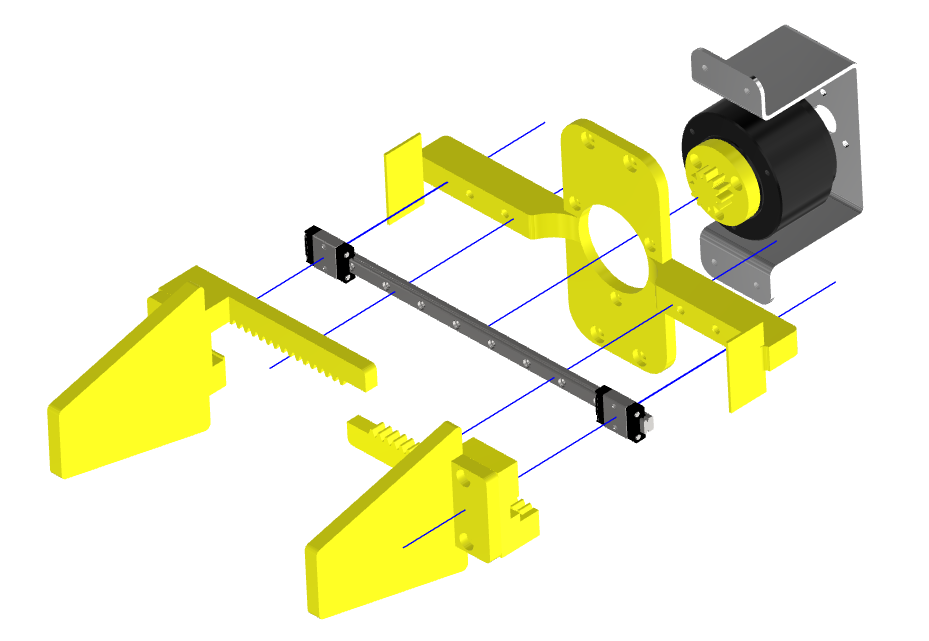
\includegraphics[width=10cm]{images/design/hand.png}
  \caption{Exploded view of parallel gripper}
  \label{fig:hand}
\end{figure}

\newpage
%
\chapter{製作}
\label{chap:production}
%
本章では,ロボットアームの製作について述べる.
製作してから書きます.
%%!TEX root = ../thesis.tex
\section{部品}
ロボットアームは,QDDモータ,アルミ板金,アルミフレーム,平行グリッパ,から構成されている.アルミ板金部品は,すべてMeviy\cite{Meviy:online}から入手できる.使用する部品のリストと購入金額を図に示す.
\begin{figure}[H]
  \centering
  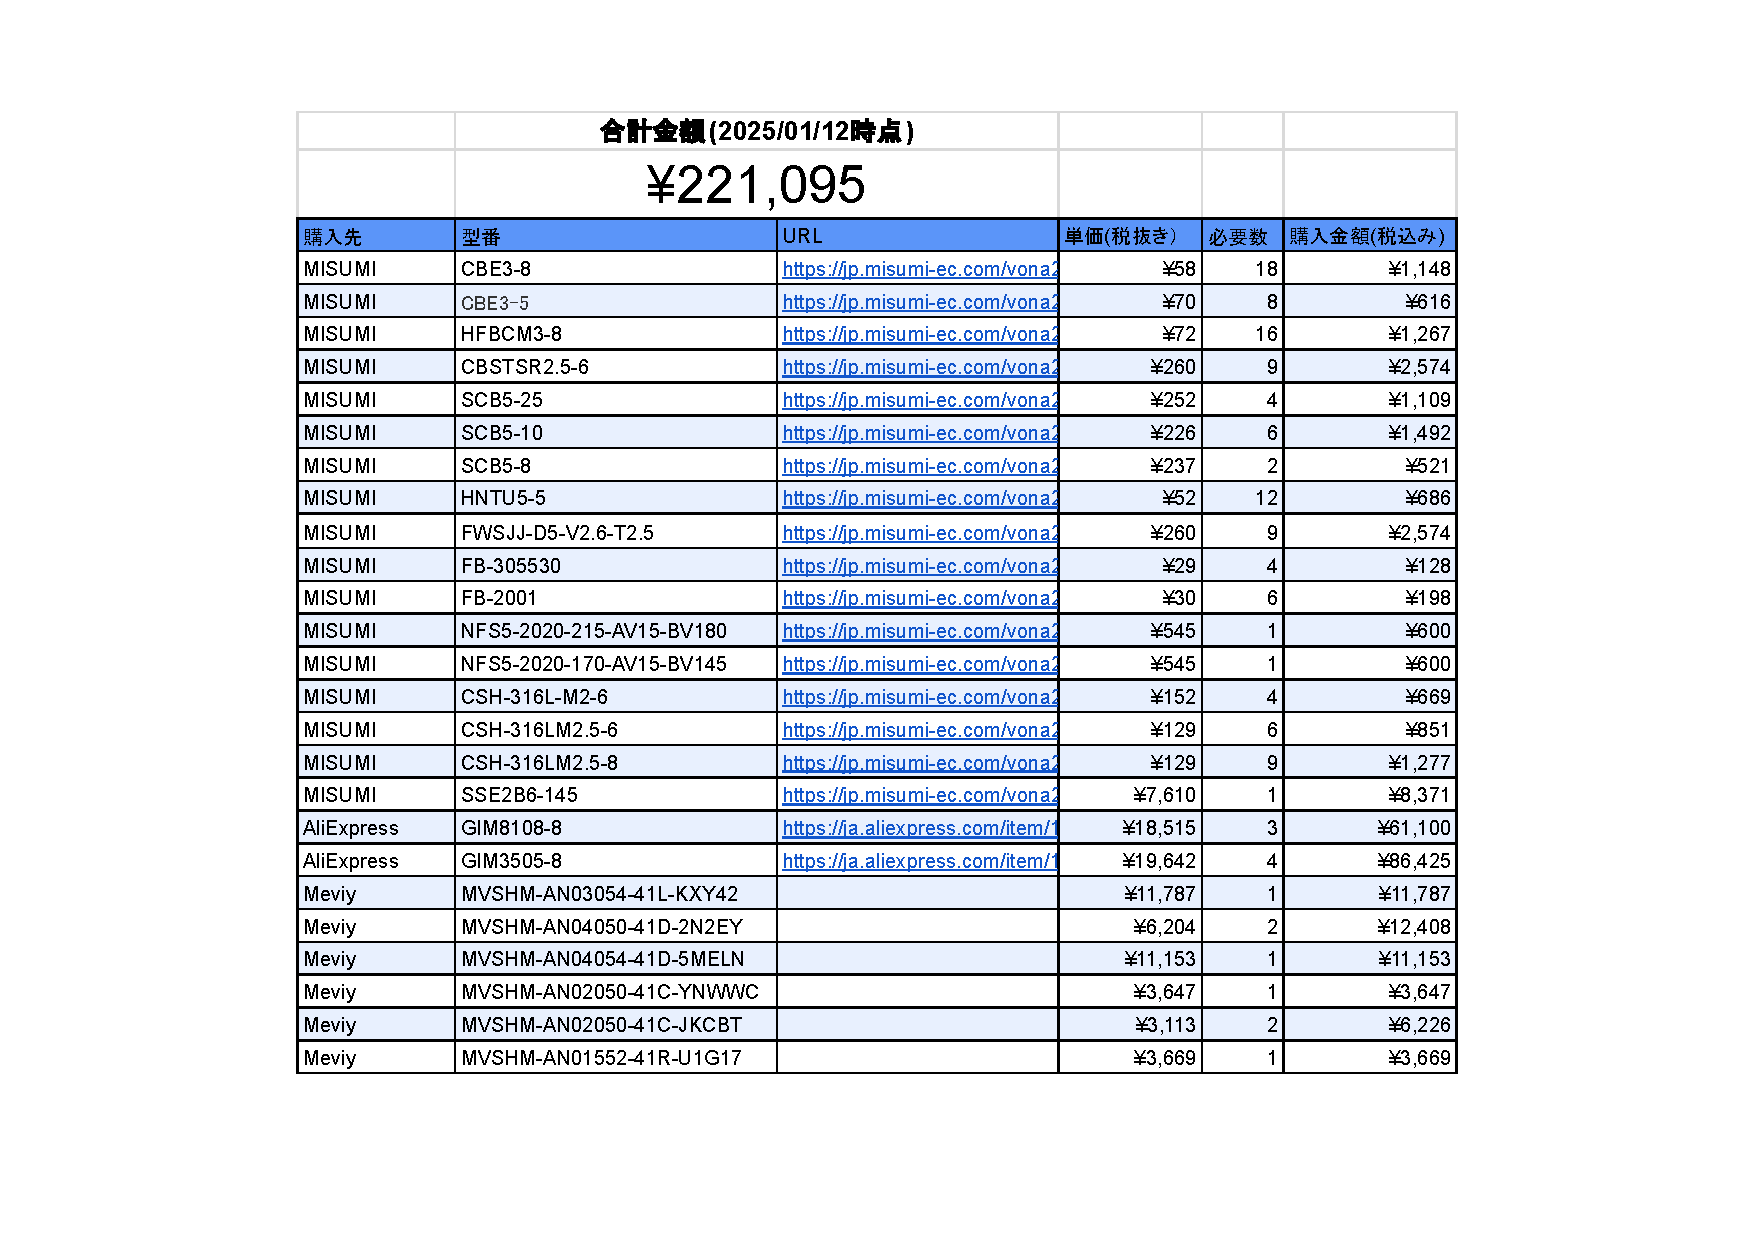
\includegraphics[width=10cm]{images/product/rist.pdf}
  \caption{部品リスト}
  \label{fig:parts}
\end{figure}
\newpage
\section{部品の製作}
\section{組み立て}
\section{安全対策}
%
\chapter{結論}
\label{chap:conclusion}
%
%!TEX root = ../thesis.tex
\section{まとめ}

\section{今後の展望}
\newpage
%
%ここにディレクトリのパスを追加していく
%
%% Back Matter
\backmatter{}
%
\chapter{設計}
\label{chap:third}
%
本章ではロボットアームのメカニズムの設計について述べる.
まず,選定したQDDモータについて説明し,ロボットアームの設計について述べる.

%!TEX root = ../thesis.tex
\section{オープンプラットフォームを意識した設計}
\newpage
%!TEX root = ../thesis.tex
\section{QDDモータの選定}
飯塚ら\cite{飯塚浩太2021}の研究では,減速比10:1のQDDモータが使用されている.また,Zhaoら\cite{10106520}の研究においては,減速比9:1のQDDモータが採用されていた.これらの先行研究は,ロボットアームと人の衝突時の衝撃力軽減を実現するためには,この程度の減速比を持つモータを採用することが有効であることを示唆している.

さらに,本研究ではオープンプラットフォームの観点を重視し,他のロボットアームに使用されているモータと同程度,またはそれ以下の価格であることを選定基準とした.調査対象としたオフィスロボットのうち,ロボットアームに使用しているアクチュエータの価格は,約3万円から約8万円であったため,価格上限を8万円に設定した.

以上を踏まえ,本研究では,持つSteadywinのGIM8108-8とGIM3505-8を採用した.減速比は8:1であり,先行研究で使用されていたモータと同程度の減速比を持つ.また,価格は約19,000円と約18,000円であり,価格上限である8万円を下回っている.
\subsection{選定したモータの性能}
表\ref{tab:QDDComparison}に,選定したQDDモータとReachy\cite{Reachy:online}のアームに使用されているモータ(Dynamixel MX-106T)の比較を示す.選定したSteadywinのGIM8108-8とGIM3505-8は,減速比が8:1で,先行研究で使用していた減速比と近しい物になっている.適切に制御することで衝突時の衝撃を軽減することが可能である.また,許容ラジアル荷重とアキシアル荷重も高いため,追加の補強部品を必要とせずにロボットアームの構造を簡略化することが可能である.
\begin{table}[]
  \centering
  \caption{QDD motor performance comparison}
  \label{tab:QDDComparison}
  \begin{tabular}{lccc}
  \hline
               & \begin{tabular}[c]{@{}c@{}}SteadyWin\\ GIM8108-8\end{tabular} & \begin{tabular}[c]{@{}c@{}}SteadyWin\\ GIM3505-8\end{tabular} & \begin{tabular}[c]{@{}c@{}}Dynamixel\\ MX-106T\end{tabular} \\ \hline
  減速比          & 8 : 1                                                         & 8 : 1                                                         & 225 : 1                                                     \\
  定格トルク(Nm)    & 7.5                                                           & 0.65                                                          & -                                                           \\
  最大トルク(Nm)    & 22                                                            & 1.27                                                          & 10                                                          \\
  重量(g)        & 396                                                           & 97                                                            & 153                                                         \\
  無負荷回転数(rpm)  & 320                                                           & 384                                                           & 55                                                          \\
  許容ラジアル荷重(N)  & 900                                                           & 300                                                           & 40                                                          \\
  許容アキシアル荷重(N) & 225                                                           & 75                                                            & 20                                                          \\
  価格(円)        & 約19,000                                                       & 約18,000                                                       & 約80,000                                                     \\ \hline
  \end{tabular}
\end{table}

\subsection{QDDモータの欠点}
QDDモータは高トルク・高スピードでの動作が可能であるという利点を持つ一方で、この特性は制御が不十分な場合にリスクとなる.特に、通電時に動作が暴走した場合、一般的なモータと比較して周囲の人や機器への被害が大きい.そのため、QDDモータを安全に運用するためには、適切な制御と安全対策が必要である.
\newpage
%!TEX root = ../thesis.tex
\section{基本的な性能}
設計したロボットアームの基本的な性能を述べる.
\subsection{アームサイズ}
図\ref{fig:link_length}にロボットアームのアームリーチとリンク長を示す.人間の腕の長さの比\cite{humanarm:online}を参考に,肩から肘までは290㎜,肘から手首までは220㎜とした.アームリーチは660㎜であり,要求仕様の700㎜程度を満たしている.図\ref{fig:arm_size}にアームサイズを示す.比較のため,机とボトルを模したものを配置している.

\begin{figure}[htbp]
  \centering
  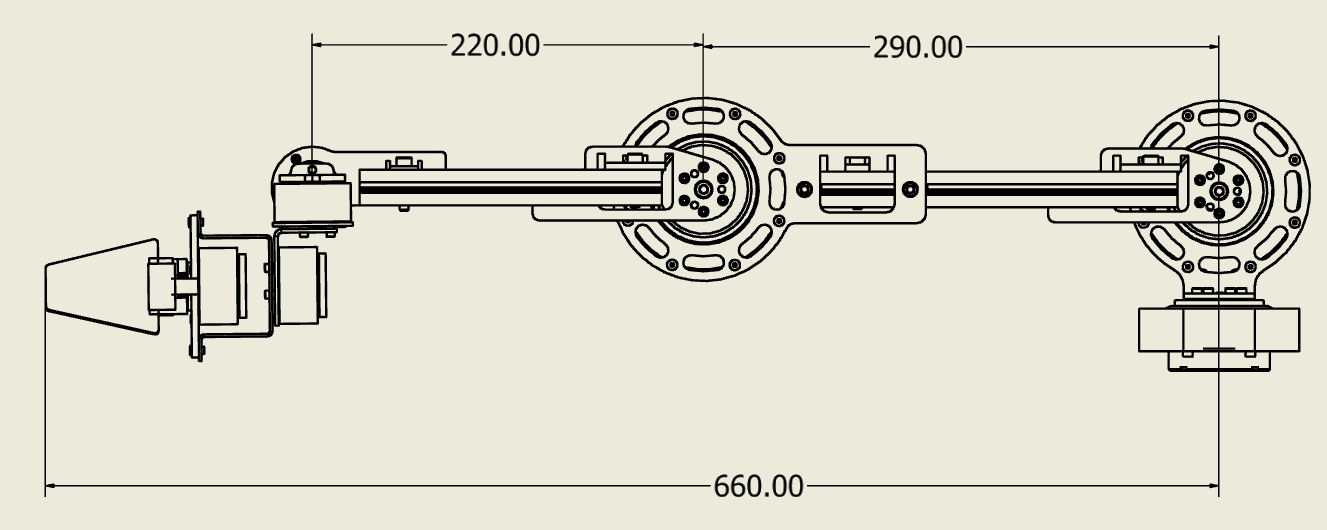
\includegraphics[width=10cm]{images/link_length.png}
  \caption{Arm reach and link length}
  \label{fig:link_length}
\end{figure}

\begin{figure}[htbp]
  \centering
  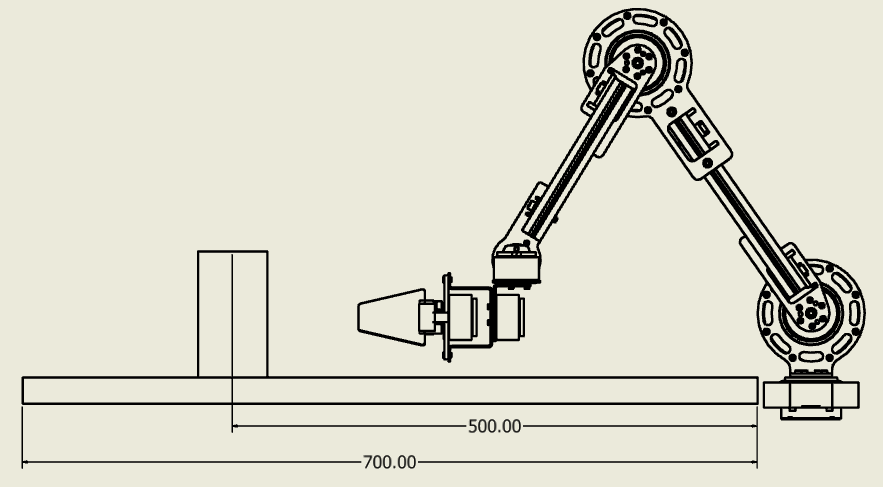
\includegraphics[width=10cm]{images/hikaku.png}
  \caption{Arm size}
  \label{fig:arm_size}
\end{figure}

\clearpage

\subsection{可動範囲}
図\ref{fig:arm_short},図\ref{fig:arm_long}にアームの最小可動範囲と最大可動範囲を示す.最小可動範囲は,アームの部品が干渉することなく動作できる最小の範囲を示しており,最大可動範囲はアームを最大まで伸ばしたときの範囲を示している.

\begin{figure}[htbp]
  \centering
  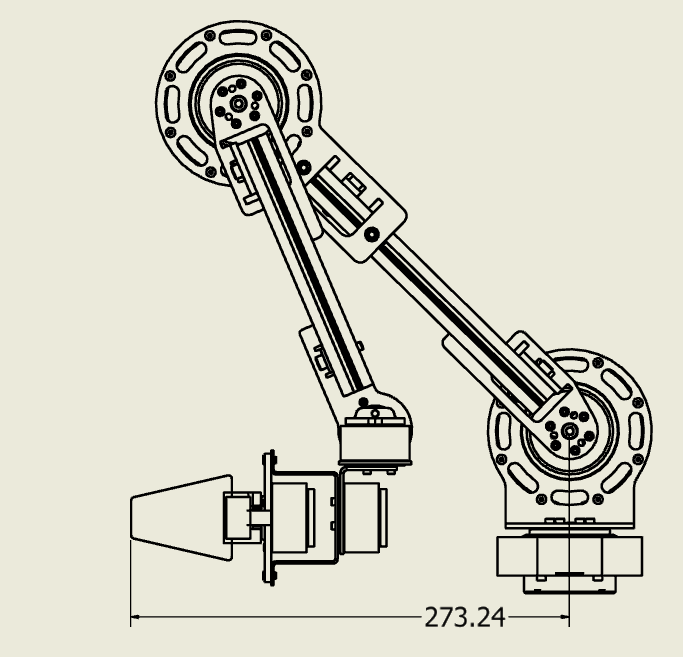
\includegraphics[width=10cm]{images/design/arm_short.png}
  \caption{Minimum range of motion}
  \label{fig:arm_short}
\end{figure}

\begin{figure}[htbp]
  \centering
  \includegraphics[width=10cm]{images/design/arm_long.png}
  \caption{Minimum range of motion}
  \label{fig:arm_long}
\end{figure}

\subsection{アームの手先の移動}
アームの手先の移動の様子を図\ref{fig:move1},図\ref{fig:move2},図\ref{fig:move3},図\ref{fig:move4}に示す.

\begin{figure}[h]
  \centering
  \includegraphics[width=10cm]{images/design/migitika.png}
  \caption{Stretched out to the right}
  \label{fig:move1}
\end{figure}

\begin{figure}[h]
  \centering
  \includegraphics[width=10cm]{images/design/migioku.png}
  \caption{Stretched out to the right}
  \label{fig:move2}
\end{figure}

\begin{figure}[h]
  \centering
  \includegraphics[width=8cm]{images/design/hidaritika.png}
  \caption{Stretched out to the left}
  \label{fig:move3}
\end{figure}

\begin{figure}[h]
  \centering
  \includegraphics[width=10cm]{images/design/hidarioku.png}
  \caption{Stretched out to the left}
  \label{fig:move4}
\end{figure}
\clearpage

\subsection{可搬重量}
肩ピッチ軸のQDDモータ(SteadyWin GIM8108-8)の定格トルクは7.5Nm,最大トルクは22Nmである.アームを伸ばしたときに自重を支えるために必要なトルクを求め,常時把持することのできる物体の重量と,瞬間的に把持することのできる物体の重量を求める.
\subsubsection{自重を支える為に必要なトルク}
図\ref{fig:CoG}にアームの重心を示す.アームの重心は肩ピッチ軸から0.334mの位置にあり,アームの重さは1.31kgである.重力加速度を9.8m/s$^2$とすると,肩ピッチ軸にかかるトルク$T$は次のように求められる.
\begin{equation}
  T = 1.31 \times 9.8 \times 0.334 = 4.2 Nm
\end{equation}
\begin{figure}[h]
  \centering
  \includegraphics[width=10cm]{images/design/CoG.png}
  \caption{Center of gravity}
  \label{fig:CoG}
\end{figure}

\subsubsection{常時把持することのできる物体の重量}
アームの定格トルクから,自重を支える為に必要なトルクを引くと3.3Nmであり,肩ピッチ軸から手先までの距離は0.66mである.したがって,常時把持することのできる物体の重量$m$は次のように求められる.
\begin{equation}
  m = 3.3 / (9.8 \times 0.66) = 0.51kg
\end{equation}

\subsubsection{瞬間的に把持することのできる物体の重量}
同様に,最大トルクから自重を支える為に必要なトルクを引くと17.8Nmである.したがって,瞬間的に把持することのできる物体の重量$M$は次のように求められる.
\begin{equation}
  m = 17.8 / (9.8 \times 0.66) = 2.75kg
\end{equation}


\clearpage
\newpage
%!TEX root = ../thesis.tex
\section{強度確認}
設計したロボットアームの強度確認のため,Autodesk Inventorの機能である構造解析を行った.解析における安全率が1以上であれば,強度が十分であると判断した.図\ref{fig:shoulder}に肩部の構成を示す.肩部は,ヨー軸モータとピッチ軸モータを繋ぐ図\ref{fig:shoulder}の部品1,およびリンクの一部である,部品2から構成されている.部品1および部品2には,いずれもアルミニウム合金(A5052)を使用している.

本節では,構造解析による部品の強度確認について述べる.

\begin{figure}[h]
  \centering
  \includegraphics[width=10cm]{images/design/shoulder.png}
  \caption{Configuration of the shoulder components}
  \label{fig:shoulder}
\end{figure}

\subsection{部品1の構造解析}
図\ref{fig:shoulder}の部品1は,ヨー軸モータが最大出力22Nmを発生した際に最大負荷を受ける部品である.図\ref{fig:T3_40}に構造解析結果を示し,設計仕様を表\ref{tab:part1_spec}にまとめた.解析の結果,安全率は0.39であり,強度が不足していることが確認された.特に,図\ref{fig:T3_40}の結果から,曲げ加工部分において強度が不足していることが明らかとなった.この課題を解決するため,「板厚を変更した部品」と「形状を変更した部品」の2つの設計案を検討し,それぞれ再解析を実施した.

\begin{figure}[h]
  \centering
  \includegraphics[width=6cm]{images/design/T3_40.png}
  \caption{Structural analysis results of Part 1}
  \label{fig:T3_40}
\end{figure}

\begin{table}[h]
  \centering
  \caption{Specifications of Part 1}
  \begin{tabular}{lc}
    \hline
    厚み & 3㎜ \\ 
    質量 & 43.6g \\ 
    安全率 & 0.39 \\ \hline
  \end{tabular}
  \label{tab:part1_spec}
\end{table}
\clearpage

\subsection{設計の変更}
部品の形状はそのままに,板厚を3mmから5mmに変更した場合の構造解析結果を図\ref{fig:T5}に示し,設計仕様を表\ref{tab:part1_spec_T5}にまとめた.解析の結果,安全率は基準の1を超え,強度が十分であることが確認された.ただし,質量が27.5g増加するという結果が得られた.

\begin{figure}[h]
  \centering
  \includegraphics[width=6cm]{images/design/T5.png}
  \caption{Structural analysis results of Part 1 (thickness changed to 5mm)}
  \label{fig:T5}
\end{figure}

\begin{table}[h]
  \centering
  \caption{Specifications of Part 1 (thickness changed to 5mm)}
  \begin{tabular}{lc}
    \hline
    厚み & 5㎜ \\ 
    質量 & 71.1g \\ 
    安全率 & 1.01 \\ \hline
  \end{tabular}
  \label{tab:part1_spec_T5}
\end{table}
\clearpage

次に,板厚を変更せず,形状の改良を行った場合の解析結果を図\ref{fig:T3_80}に示し,設計仕様を表\ref{tab:part1_spec_T3_80}にまとめた.具体的には,図\ref{fig:T3_40}の解析結果を基に,特に強度が不足していると判明した曲げ加工部分の幅を広げる設計変更を行った.

解析の結果,安全率が基準を満たし,十分な強度を確保できることが確認された.また,重量は61.8gであり,板厚を変更した場合(表\ref{tab:part1_spec_T5}参照)と比較して軽量化を実現した.

以上の解析結果を踏まえ,図\ref{fig:shoulder}の部品1について,曲げ加工部分の幅を広げた設計変更を最終設計として採用した.

\begin{figure}[h]
  \centering
  \includegraphics[width=6cm]{images/design/T3_80.png}
  \caption{Structural analysis results of Part 1 (shape optimized)}
  \label{fig:T3_80}
\end{figure}

\begin{table}[h]
  \centering
  \caption{Specifications of Part 1 (shape optimized)}
  \begin{tabular}{lc}
    \hline
    厚み & 3㎜ \\ 
    質量 & 61.8g \\ 
    安全率 & 1.1 \\ \hline
  \end{tabular}
  \label{tab:part1_spec_T3_80}
\end{table}

\subsection{部品2の構造解析}
図\ref{fig:shoulder}の部品2は,アルミフレームを2方向から固定する形状を採用している(図\ref{fig:pitchalumi}参照).最大負荷条件(22Nm)の下で構造解析を実施した結果を図\ref{fig:pitch}に示す.現行の設計では,安全率が0.47と低く,特に赤色で示された箇所において強度不足が確認された.

\begin{figure}[h]
  \centering
  \includegraphics[width=6cm]{images/design/pitchlink.png}
  \caption{Fixing the aluminum frame and part 2}
  \label{fig:pitchalumi}
\end{figure}

\begin{figure}[h]
  \centering
  \includegraphics[width=6cm]{images/design/pitch.png}
  \caption{Structural analysis results of Part 2 at maximum output of 22Nm}
  \label{fig:pitch}
\end{figure}

部品の厚みを5mmに変更した場合,安全率は0.58に改善したものの,依然として基準に満たなかった.このため,定格出力(7.5Nm)の条件下で再解析を実施した.解析結果を図\ref{fig:pitchok}に示し,設計仕様を表\ref{tab:part2_spec}にまとめた.この結果,定格条件下では安全率が基準を満たし,十分な強度を確保できることが確認された.

以上より,現設計において部品2の形状変更は行わないこととし,最大出力時の安全率の確保を今後の課題とする.
\begin{figure}[h]
  \centering
  \includegraphics[width=6cm]{images/design/pitchok.png}
  \caption{Structural analysis results of Part 2 at rated output 7.5Nm}
  \label{fig:pitchok}
\end{figure}
\begin{table}[h]
  \centering
  \caption{Specifications of Part 2}
  \begin{tabular}{lc}
    \hline
    厚み & 5㎜ \\ 
    質量 & 34.0g \\ 
    安全率 & 1.38 \\ \hline
  \end{tabular}
  \label{tab:part2_spec}
\end{table}

\newpage
%!TEX root = ../thesis.tex
\section{平行グリッパの設計}
本研究では,リニアガイドとラック&ピニオン機構を用いた平行グリッパを設計した.図\ref{fig:hand}は平行グリッパの分解図である.グリッパの開閉には,QDDモータ(Steadywin GIM3505-8)を使用し,モータに取り付けたギアを介してラック&ピニオン機構で駆動する.グリッパのスライド部分にはリニアガイドを採用している.また,黄色の部品は3Dプリンタでの製作を行う.
\begin{figure}[htbp]
  \centering
  \includegraphics[width=10cm]{images/design/hand.png}
  \caption{Exploded view of parallel gripper}
  \label{fig:hand}
\end{figure}

\newpage
%
%

\end{document}